\documentclass[]{article}
\usepackage{lmodern}
\usepackage{amssymb,amsmath}
\usepackage{ifxetex,ifluatex}
\usepackage{fixltx2e} % provides \textsubscript
\ifnum 0\ifxetex 1\fi\ifluatex 1\fi=0 % if pdftex
  \usepackage[T1]{fontenc}
  \usepackage[utf8]{inputenc}
\else % if luatex or xelatex
  \ifxetex
    \usepackage{mathspec}
  \else
    \usepackage{fontspec}
  \fi
  \defaultfontfeatures{Ligatures=TeX,Scale=MatchLowercase}
\fi
% use upquote if available, for straight quotes in verbatim environments
\IfFileExists{upquote.sty}{\usepackage{upquote}}{}
% use microtype if available
\IfFileExists{microtype.sty}{%
\usepackage{microtype}
\UseMicrotypeSet[protrusion]{basicmath} % disable protrusion for tt fonts
}{}
\usepackage[margin=1in]{geometry}
\usepackage{hyperref}
\hypersetup{unicode=true,
            pdftitle={Untitled},
            pdfauthor={JingjingQi},
            pdfborder={0 0 0},
            breaklinks=true}
\urlstyle{same}  % don't use monospace font for urls
\usepackage{color}
\usepackage{fancyvrb}
\newcommand{\VerbBar}{|}
\newcommand{\VERB}{\Verb[commandchars=\\\{\}]}
\DefineVerbatimEnvironment{Highlighting}{Verbatim}{commandchars=\\\{\}}
% Add ',fontsize=\small' for more characters per line
\usepackage{framed}
\definecolor{shadecolor}{RGB}{248,248,248}
\newenvironment{Shaded}{\begin{snugshade}}{\end{snugshade}}
\newcommand{\KeywordTok}[1]{\textcolor[rgb]{0.13,0.29,0.53}{\textbf{#1}}}
\newcommand{\DataTypeTok}[1]{\textcolor[rgb]{0.13,0.29,0.53}{#1}}
\newcommand{\DecValTok}[1]{\textcolor[rgb]{0.00,0.00,0.81}{#1}}
\newcommand{\BaseNTok}[1]{\textcolor[rgb]{0.00,0.00,0.81}{#1}}
\newcommand{\FloatTok}[1]{\textcolor[rgb]{0.00,0.00,0.81}{#1}}
\newcommand{\ConstantTok}[1]{\textcolor[rgb]{0.00,0.00,0.00}{#1}}
\newcommand{\CharTok}[1]{\textcolor[rgb]{0.31,0.60,0.02}{#1}}
\newcommand{\SpecialCharTok}[1]{\textcolor[rgb]{0.00,0.00,0.00}{#1}}
\newcommand{\StringTok}[1]{\textcolor[rgb]{0.31,0.60,0.02}{#1}}
\newcommand{\VerbatimStringTok}[1]{\textcolor[rgb]{0.31,0.60,0.02}{#1}}
\newcommand{\SpecialStringTok}[1]{\textcolor[rgb]{0.31,0.60,0.02}{#1}}
\newcommand{\ImportTok}[1]{#1}
\newcommand{\CommentTok}[1]{\textcolor[rgb]{0.56,0.35,0.01}{\textit{#1}}}
\newcommand{\DocumentationTok}[1]{\textcolor[rgb]{0.56,0.35,0.01}{\textbf{\textit{#1}}}}
\newcommand{\AnnotationTok}[1]{\textcolor[rgb]{0.56,0.35,0.01}{\textbf{\textit{#1}}}}
\newcommand{\CommentVarTok}[1]{\textcolor[rgb]{0.56,0.35,0.01}{\textbf{\textit{#1}}}}
\newcommand{\OtherTok}[1]{\textcolor[rgb]{0.56,0.35,0.01}{#1}}
\newcommand{\FunctionTok}[1]{\textcolor[rgb]{0.00,0.00,0.00}{#1}}
\newcommand{\VariableTok}[1]{\textcolor[rgb]{0.00,0.00,0.00}{#1}}
\newcommand{\ControlFlowTok}[1]{\textcolor[rgb]{0.13,0.29,0.53}{\textbf{#1}}}
\newcommand{\OperatorTok}[1]{\textcolor[rgb]{0.81,0.36,0.00}{\textbf{#1}}}
\newcommand{\BuiltInTok}[1]{#1}
\newcommand{\ExtensionTok}[1]{#1}
\newcommand{\PreprocessorTok}[1]{\textcolor[rgb]{0.56,0.35,0.01}{\textit{#1}}}
\newcommand{\AttributeTok}[1]{\textcolor[rgb]{0.77,0.63,0.00}{#1}}
\newcommand{\RegionMarkerTok}[1]{#1}
\newcommand{\InformationTok}[1]{\textcolor[rgb]{0.56,0.35,0.01}{\textbf{\textit{#1}}}}
\newcommand{\WarningTok}[1]{\textcolor[rgb]{0.56,0.35,0.01}{\textbf{\textit{#1}}}}
\newcommand{\AlertTok}[1]{\textcolor[rgb]{0.94,0.16,0.16}{#1}}
\newcommand{\ErrorTok}[1]{\textcolor[rgb]{0.64,0.00,0.00}{\textbf{#1}}}
\newcommand{\NormalTok}[1]{#1}
\usepackage{graphicx,grffile}
\makeatletter
\def\maxwidth{\ifdim\Gin@nat@width>\linewidth\linewidth\else\Gin@nat@width\fi}
\def\maxheight{\ifdim\Gin@nat@height>\textheight\textheight\else\Gin@nat@height\fi}
\makeatother
% Scale images if necessary, so that they will not overflow the page
% margins by default, and it is still possible to overwrite the defaults
% using explicit options in \includegraphics[width, height, ...]{}
\setkeys{Gin}{width=\maxwidth,height=\maxheight,keepaspectratio}
\IfFileExists{parskip.sty}{%
\usepackage{parskip}
}{% else
\setlength{\parindent}{0pt}
\setlength{\parskip}{6pt plus 2pt minus 1pt}
}
\setlength{\emergencystretch}{3em}  % prevent overfull lines
\providecommand{\tightlist}{%
  \setlength{\itemsep}{0pt}\setlength{\parskip}{0pt}}
\setcounter{secnumdepth}{0}
% Redefines (sub)paragraphs to behave more like sections
\ifx\paragraph\undefined\else
\let\oldparagraph\paragraph
\renewcommand{\paragraph}[1]{\oldparagraph{#1}\mbox{}}
\fi
\ifx\subparagraph\undefined\else
\let\oldsubparagraph\subparagraph
\renewcommand{\subparagraph}[1]{\oldsubparagraph{#1}\mbox{}}
\fi

%%% Use protect on footnotes to avoid problems with footnotes in titles
\let\rmarkdownfootnote\footnote%
\def\footnote{\protect\rmarkdownfootnote}

%%% Change title format to be more compact
\usepackage{titling}

% Create subtitle command for use in maketitle
\providecommand{\subtitle}[1]{
  \posttitle{
    \begin{center}\large#1\end{center}
    }
}

\setlength{\droptitle}{-2em}

  \title{Untitled}
    \pretitle{\vspace{\droptitle}\centering\huge}
  \posttitle{\par}
    \author{JingjingQi}
    \preauthor{\centering\large\emph}
  \postauthor{\par}
      \predate{\centering\large\emph}
  \postdate{\par}
    \date{3/18/2020}


\begin{document}
\maketitle

\subsubsection{1. Wrangling scRNA-seq data in R using bioconductor
packages. (11 pts total plus 2 extra-credit points
possible)}\label{wrangling-scrna-seq-data-in-r-using-bioconductor-packages.-11-pts-total-plus-2-extra-credit-points-possible}

Download the count matrix (WT-1.dge.txt.gz) and read it into R.\\
Note: given the size of the matrix, you may have to do the analysis on
the server, where you will not have access to RStudio, but to the
console (just type R after logging in and switching to your designated
folder). To obtain images for your Rmarkdown report, you could, for
example, opt to write and compile the Rmd on your laptop. This would
mean that you should set the chunk options to eval=FALSE because you're
not going to actually execute the code on your machine. To include
images this way, you would have to compute them on the server, download
them via scp and integrate them into the report via the common markdown
syntax: \includegraphics{path-to-image}. For more info on code chunks,
see here. ALTERNATIVELY, without changing the chunk options, you could
compile the html on the server where rmarkdown::render(``input.Rmd'')
(within R) will carry out the rendering that happens when you click
``Knit'' in RStudio.

\begin{Shaded}
\begin{Highlighting}[]
\NormalTok{df <-}\StringTok{ }\KeywordTok{read.delim}\NormalTok{(}\StringTok{"WT-1.dge.txt"}\NormalTok{)}
\end{Highlighting}
\end{Shaded}

\begin{Shaded}
\begin{Highlighting}[]
\KeywordTok{head}\NormalTok{(df)}
\end{Highlighting}
\end{Shaded}

\begin{verbatim}
##        GENE GGTCCAGATCAT CCCCCATTATGC TTTACCTAACAG ATTCCCGAGTCA
## 1      A1BG            0            0            0            0
## 2  A1BG-AS1            0            0            0            0
## 3     A2ML1            0            0            0            0
## 4 A2ML1-AS1            0            0            0            0
## 5 A2ML1-AS2            0            0            0            0
## 6    A4GALT            0            0            0            0
##   ATTCATTCTTTG GTCTTCTCCCAT CCGCTACTTCTC TTCCAGCCTCGG CGCTACACTGGA
## 1            0            0            0            0            0
## 2            0            0            0            0            0
## 3            0            1            0            0            0
## 4            0            0            0            0            0
## 5            0            0            0            0            0
## 6            0            0            0            0            0
##   TTCGCTGAAAAC GATTTTACTTGT ACTAAGTAAGCT TCCTGGCCACGA GTTTTCTACAGC
## 1            0            0            0            0            0
## 2            0            0            0            0            0
## 3            0            0            0            0            0
## 4            0            0            0            0            0
## 5            0            0            0            0            0
## 6            0            3            0            0            0
##   GCTCTGGCCAAT CCGTCTGGTGAC TGTCAATCCGTA CACTTTCTTGTC CTAGTAGCAGTT
## 1            0            0            0            0            0
## 2            0            0            0            0            0
## 3            0            0            0            0            0
## 4            0            0            0            0            0
## 5            0            0            0            0            0
## 6            0            0            0            0            0
##   ATAATGACGGCT GCCTCGAACACT TCCACCCGACTG TTCTCATCTATC TTGTTAAAGTCC
## 1            0            0            0            0            0
## 2            0            1            0            0            0
## 3            0            0            0            0            0
## 4            0            0            0            0            0
## 5            0            0            0            0            0
## 6            0            0            0            0            0
##   CTATGGTCTTCT TAGTTTCCATTG CCGTACAGCCAC GCTTTCTTTGAT CATTACGAGTGG
## 1            0            0            0            0            0
## 2            0            0            0            0            0
## 3            0            0            0            0            0
## 4            0            0            0            0            0
## 5            0            0            0            0            0
## 6            0            1            0            0            0
##   ACTCTTCCCTGT CCGTCACAATAC CCCTCTTCTCAG TATCGAGGAATT AGTTTCCCCTCA
## 1            0            0            0            0            0
## 2            0            0            0            0            0
## 3            0            0            0            0            0
## 4            0            0            0            0            0
## 5            0            0            0            0            0
## 6            0            0            0            0            0
##   TCGCTTTTGTTG TTTCACCAATAA TTTTCCGGGTGA ATCATCCAGAGC TCTTGGTCGTCA
## 1            0            0            0            0            0
## 2            0            0            0            0            0
## 3            0            0            0            0            0
## 4            0            0            0            0            0
## 5            0            0            0            0            0
## 6            0            0            0            0            1
##   AACTTCACATAA TTCCGCCCTGTA ACTCCGACCAAG GTCAATGACGAG CTGAGTGTGCCC
## 1            0            0            0            0            0
## 2            0            0            0            0            0
## 3            0            0            1            0            0
## 4            0            0            0            0            0
## 5            0            0            0            0            0
## 6            0            0            0            0            0
##   GGCTACCACCCG TATTTCGCCAGC TAATGCTCCTGC GTTTATGCCGCC TCACTATTCGGA
## 1            0            0            0            0            0
## 2            0            0            1            0            0
## 3            0            0            0            0            0
## 4            0            0            0            0            0
## 5            0            0            0            0            0
## 6            0            0            1            0            0
##   GTGTCGCAAGAA TCTGTTGGGACG CAGCTCATGAAT GTCCTTATTCAG GTACCTACGCGA
## 1            0            0            0            0            0
## 2            0            0            0            1            0
## 3            0            0            0            0            0
## 4            0            0            0            0            0
## 5            0            0            0            0            0
## 6            0            0            0            1            0
##   CTACAGTCGTTT GCTCCTCCCCGN GATTGGGTTTTT CAGCCTTCTAGA ACAGCTGAAGCG
## 1            0            0            0            0            0
## 2            0            0            0            0            0
## 3            0            0            1            0            0
## 4            1            0            0            0            0
## 5            0            0            0            0            0
## 6            0            0            0            0            0
##   GACTTGGGGACN CCCTACTTTTTG CCATGAGCATAA TCCACAGACAGC CAAGCAGACGTG
## 1            0            0            0            0            0
## 2            0            0            0            0            0
## 3            0            0            0            0            0
## 4            0            0            0            0            0
## 5            0            0            0            0            0
## 6            0            0            0            0            0
##   CATTATGATACT ACTTTTACTTAT TTTTAGTCAATG AACGTGGCGCCC ATTCGTCGCAGT
## 1            0            0            0            0            0
## 2            0            0            0            0            0
## 3            0            0            0            0            0
## 4            0            0            0            0            0
## 5            0            0            0            0            0
## 6            0            0            0            0            0
##   AATGCCCGTTTT TTCTCCTTGCGA ATCACGGCCTTA CTAATTCAGGAN ATCAGAAGCATA
## 1            0            0            0            0            0
## 2            0            0            0            0            1
## 3            0            0            0            0            0
## 4            0            0            0            0            0
## 5            0            0            0            0            0
## 6            0            0            0            0            0
##   TGCCAACACAAT TTACCGCTGTAA ACTTTACTCGGT CTGTATCTGCAC CTACGGCACCTT
## 1            0            0            0            0            0
## 2            0            0            0            0            0
## 3            0            0            0            0            0
## 4            0            0            0            0            0
## 5            0            0            0            0            0
## 6            0            1            0            0            0
##   TATTGATGGCTC TCCTTGGTCGGT CCTTTTGTTGTG CTCTCCGGCTGN GCGTCGTTCTGA
## 1            0            0            1            0            0
## 2            0            0            0            0            0
## 3            0            1            0            0            0
## 4            0            0            0            0            0
## 5            0            0            0            0            0
## 6            0            0            0            0            0
##   CATATCCCCCTC TAATAACACCAN CCCTATTACACG CACGTGTCAGAA ACTTATCCTCTT
## 1            0            0            0            0            0
## 2            0            0            0            0            0
## 3            0            0            0            0            0
## 4            0            0            0            0            0
## 5            0            0            0            0            0
## 6            0            0            0            0            0
##   ACGTCGGGCGGT TTTAACAATTGC GAATTAGATAGC GGCCCTATTGAA ACTTGGTGTAGA
## 1            0            0            0            0            0
## 2            0            0            0            0            0
## 3            0            0            0            0            0
## 4            0            0            0            0            0
## 5            0            0            0            0            0
## 6            0            0            0            0            1
##   TGTTTATATGGA TTGCTCCTCCTT GCCCCCGTGCTT CTGAAGCAGTTA TTATTCGGGCTN
## 1            0            0            0            0            0
## 2            0            0            0            0            0
## 3            0            0            0            0            0
## 4            0            0            0            0            0
## 5            0            0            0            0            0
## 6            0            1            0            0            0
##   CTATGGGAACGC ATCTCCCGCCGT AGCTTGTAAATC GCTCACTGACTA TGTTCTCATTAT
## 1            0            0            0            0            0
## 2            0            0            0            0            0
## 3            0            0            0            0            0
## 4            0            0            0            0            0
## 5            0            0            0            0            0
## 6            0            0            0            0            0
##   CGCCATGATTTG ATCGAGTATTCT CTTCGAATCCCA ACCGTTGGGTCC GTGTTTCCCAAT
## 1            0            0            0            0            0
## 2            0            0            0            0            0
## 3            0            0            0            0            0
## 4            0            0            0            0            0
## 5            0            0            0            0            0
## 6            0            0            0            0            0
##   CCCCGAAACTAA GTATGCGTAAGT AGTACATCGCTG AAAAACTTGGTN CGGCGCAAGGCA
## 1            0            0            0            0            0
## 2            0            0            0            0            0
## 3            0            0            0            0            0
## 4            0            0            0            0            0
## 5            0            0            0            0            0
## 6            0            0            0            0            0
##   GATCATTCTGGT CGATCACGTTTG CTCGCTCCTCGT CTGGAACATAAA TCTGTAATTGAC
## 1            0            0            0            0            0
## 2            0            0            0            0            0
## 3            0            0            0            0            0
## 4            0            0            0            0            0
## 5            0            0            0            0            0
## 6            0            0            0            0            0
##   ATTTAAGTCAAA CATTGCACGCCA CATTTCATTGCA TTTTTAATGCAN CTTTACGCGCGT
## 1            0            0            0            0            0
## 2            0            0            0            0            0
## 3            0            0            0            0            0
## 4            0            0            0            0            0
## 5            0            0            0            0            0
## 6            0            1            0            0            0
##   GAATCTGTTTTT TCATAATTTGAT TCATCAGAGACC GTTCCCGAGTCA CTGTAGCGCCTG
## 1            0            0            0            0            0
## 2            0            0            0            0            0
## 3            0            0            0            0            0
## 4            0            0            0            0            0
## 5            0            0            0            0            0
## 6            0            0            0            0            0
##   GCCACGCTGTGN GAATTGCCTTGG GTCTTCTCCACG ATCGCGGCTCCT GTGACGGGACGC
## 1            0            0            0            0            0
## 2            0            0            0            0            0
## 3            0            0            0            0            1
## 4            0            0            0            0            0
## 5            0            0            0            0            0
## 6            0            1            0            0            0
##   TGTCCCACATCA GTTTTGGGTATC AGATTTACCCGT CTGCTCTATAAN CCAAGTGACATA
## 1            0            0            0            0            0
## 2            0            0            0            0            0
## 3            0            2            0            0            0
## 4            0            0            0            0            0
## 5            0            0            0            0            0
## 6            0            0            0            0            0
##   CTATTTAACAGA TAGGCACCTCGN ATCCATGTGACT CGTCACTCAGTC ATTGATGCCGCC
## 1            0            0            0            0            0
## 2            0            0            0            0            0
## 3            0            0            0            0            0
## 4            0            0            0            0            0
## 5            0            0            0            0            0
## 6            0            0            0            0            0
##   AGAACGCACAAA ACATGTCAGTTA ACTTCGGCATGT TTCCTCATAATT TCATACACCCGT
## 1            0            0            2            0            0
## 2            0            0            0            0            0
## 3            0            0            0            0            0
## 4            0            0            0            0            0
## 5            0            0            0            0            0
## 6            0            0            0            0            0
##   GCCGATAACAAG AACCTCCTGAGA GTGTAATGGTAT TATCTTCCAGAA ACCGATTTACAA
## 1            0            0            0            0            0
## 2            0            0            0            0            0
## 3            0            0            0            0            0
## 4            0            0            0            0            0
## 5            0            0            0            0            0
## 6            0            0            0            0            0
##   GTCGTGCCCTAT CTAACCAGCGAG ACCACAATCCCG ATTGCTCTCACT ATCGCCCGGCGC
## 1            0            0            0            0            0
## 2            0            0            0            0            0
## 3            0            0            0            0            0
## 4            0            0            0            0            0
## 5            0            0            0            0            0
## 6            0            0            0            0            0
##   AATACGTTAAGC TAGCTGGGCGTG ACATCTGATTTT GTACATACCCCT TTTGCAGCGGGN
## 1            0            0            0            0            0
## 2            0            0            0            0            0
## 3            0            0            0            0            0
## 4            0            0            0            0            0
## 5            0            0            0            0            0
## 6            0            0            0            0            0
##   TGTTTATAGTGC GTGTTCTCGGCT CTACGCCGAATT TGTATTCATGTC CTCCGTAAATCC
## 1            0            0            0            0            0
## 2            0            0            0            0            0
## 3            0            0            0            0            0
## 4            0            0            0            0            0
## 5            0            0            0            0            0
## 6            0            0            0            0            0
##   GTTACGGACAAT CAGCATAGTCTA CAAACATACTGC CAATTAGATCGN TCGTGTATCCTC
## 1            0            0            0            0            0
## 2            0            0            0            0            0
## 3            0            0            0            0            0
## 4            0            0            0            0            0
## 5            0            0            0            0            0
## 6            0            0            0            0            0
##   CATACTATGGAA GTATTCCCGATG CAGTAGCCTGGA GCTAAGTAAGCT GTTCATTCTTTG
## 1            0            0            0            0            0
## 2            0            0            0            0            0
## 3            0            0            0            0            0
## 4            0            0            0            0            0
## 5            0            0            0            0            0
## 6            0            0            0            0            0
##   CGCTTAGGTGGT TTTCCGTTTTTT ACACTTAAGTAN GTTAACGTGCAC GAGTCTCGTCCC
## 1            0            0            0            0            0
## 2            0            0            0            0            0
## 3            0            0            0            0            0
## 4            0            0            0            0            0
## 5            0            0            0            0            0
## 6            0            0            0            0            0
##   TAGAATAATTGG GGTTTTACTTGT GTTATATGAAAC TACGATCGATAC TGGTTGTTTCGT
## 1            0            0            0            0            0
## 2            0            0            0            0            0
## 3            0            0            0            0            0
## 4            0            0            0            0            0
## 5            0            0            0            0            0
## 6            0            0            0            0            0
##   ATATATGCCCCC CTTAATTGCCTA GACCAGGACTGT TAGATCCGAGCA CAATAAGGACAG
## 1            0            0            0            0            0
## 2            1            0            0            0            0
## 3            0            0            0            0            0
## 4            0            0            0            0            0
## 5            0            0            0            0            0
## 6            0            0            0            0            0
##   AAATACTGCCGC CGGGCCCACGGG GCTCTTCCCTGT AGCCCTTCGTGA AACGCTTCGTCG
## 1            0            0            0            1            0
## 2            0            0            0            0            0
## 3            0            0            0            0            0
## 4            0            0            0            0            0
## 5            0            0            0            0            0
## 6            0            0            0            0            0
##   CTAATCAGGGGA ACGTCCTCATTA GTCGGAGCCTTC ACAGTTGAGTTG CTAGACAGCGAG
## 1            0            0            0            0            0
## 2            0            0            0            0            0
## 3            0            0            0            0            0
## 4            0            0            0            0            0
## 5            0            0            0            0            0
## 6            0            0            0            0            0
##   TTAAATGATAAA GAGACGAGCTTA CCGAAGGACCAT TCCGCATTTGAC GCCTTTAGGATG
## 1            0            0            0            0            0
## 2            0            0            0            0            0
## 3            0            0            0            0            0
## 4            0            0            0            0            0
## 5            0            0            0            0            0
## 6            0            0            0            0            0
##   ACCATGGGCTCA GTTTTTGTTAAG CAGCCTCAATGT CGTCTGATTCAT TTAGTCTGAGTC
## 1            0            0            0            0            0
## 2            0            0            0            0            0
## 3            0            0            0            0            0
## 4            0            0            0            0            0
## 5            0            0            0            0            0
## 6            0            0            0            0            0
##   CGCAGGAATCTG GATAACGTCCCG GTTTGCCTGGGT ACGGCCGGCTAG ACCTAGCTGTCG
## 1            0            0            0            0            0
## 2            0            0            0            0            0
## 3            0            0            0            0            0
## 4            0            0            0            0            0
## 5            0            0            0            0            0
## 6            0            0            0            0            0
##   ACGTAACTATGC TCGGCAAACGCT GATTTAAGACCT GTGCATCCGTTG ATCCCTGCGCGC
## 1            0            0            0            0            0
## 2            0            0            0            0            0
## 3            1            0            0            0            0
## 4            0            0            0            0            0
## 5            0            0            0            0            0
## 6            0            0            0            0            0
##   TCCTTGGAGGAC ATCACACCCGTG GAGCTTGTTTGC TGCTTCCTTATC ATGTGGCCACAG
## 1            0            0            0            0            0
## 2            0            0            0            0            0
## 3            0            0            0            0            0
## 4            0            0            0            0            0
## 5            0            0            0            0            0
## 6            0            0            0            0            0
##   CAAAGCGAACAA CCTGTAAAAGAT ATGTTCGTACGT CATTATACTAGT CAGGTCATTACC
## 1            0            0            0            0            0
## 2            0            0            0            0            0
## 3            0            0            0            0            0
## 4            0            0            0            0            0
## 5            0            0            0            0            0
## 6            0            0            0            0            0
##   ACGCTTACAAGG GTCATCCAGAGC AGGGCCGCATAT CCCGCTCGCTTT CAGGTCCCACGC
## 1            0            0            0            0            0
## 2            0            0            0            0            0
## 3            0            0            0            0            0
## 4            0            0            0            0            0
## 5            0            0            0            0            0
## 6            0            0            0            0            0
##   ACCGATGATGGC TAAATAAATCAT CCTGAGGTACAC TATAGGCACTCC ACACACCCCTGC
## 1            0            0            0            0            0
## 2            0            0            0            0            0
## 3            0            0            0            0            0
## 4            0            0            0            0            0
## 5            0            0            0            0            0
## 6            0            0            0            0            0
##   TGCATCACAACT TTTCATTAATAA AGCTTGACTATG GCTCACGTAACA ACTCCTCGGTCA
## 1            0            0            0            0            0
## 2            0            0            0            0            0
## 3            0            0            0            0            0
## 4            0            0            0            0            0
## 5            0            0            0            0            0
## 6            0            0            0            0            0
##   GTAGAAGGCCGC ACATGAGCACCC GACCCGGTTGCC GTTCCCGCATAN TAGTTATCGCAT
## 1            0            0            0            0            0
## 2            0            0            0            0            0
## 3            0            0            0            0            0
## 4            0            0            0            0            0
## 5            0            0            0            0            0
## 6            0            0            0            0            0
##   TTAGGTAGTTCA GCTCCGACCAAG CGCTTTCTTGTC ACGTGCCATGCC CTCTCGTGCAAN
## 1            0            0            0            0            0
## 2            0            0            0            0            0
## 3            0            0            0            0            0
## 4            0            0            0            0            0
## 5            0            0            0            0            0
## 6            0            0            0            0            0
##   ATAGAGGTGCAC GAGCTGCCAGAA TACCCAGTAGCC CCGGCGTGTTTT GTTACATCTACA
## 1            0            0            0            0            0
## 2            0            0            0            0            0
## 3            0            0            0            0            0
## 4            0            0            0            0            0
## 5            0            0            0            0            0
## 6            0            0            0            0            0
##   CTGGTTAGCTCT CCGTATACATTG TTACCCTGCGGG CTTCGACCGTTT ATGCCGATTGCT
## 1            0            0            0            0            0
## 2            0            0            0            0            0
## 3            0            0            0            0            0
## 4            0            0            0            0            0
## 5            0            0            0            0            0
## 6            0            0            0            0            0
##   AACCAAGAAATN GGTCAGCCAACG CTTGAGCGCGTC ATTTCTCGATTT TTCTTTTCAGAC
## 1            0            0            0            0            0
## 2            0            0            0            0            0
## 3            0            1            0            0            0
## 4            0            0            0            0            0
## 5            0            0            0            0            0
## 6            0            0            0            0            0
##   TGGATACGGAGN TCCTCGTGTAAA GCTTTACTCGGT TGAATTCGACAA AGACCCGGTGGA
## 1            0            0            0            0            0
## 2            0            0            0            0            0
## 3            0            0            0            0            0
## 4            0            0            0            0            0
## 5            0            0            0            0            0
## 6            0            0            0            0            0
##   GAAAGTTGTCGT GCCCGGAGGGGC CGCCACGCTTAC TTGAGTACATTT ACTCCGAAGGCA
## 1            0            0            0            0            0
## 2            0            0            0            0            0
## 3            0            0            0            0            0
## 4            0            0            0            0            0
## 5            0            0            0            0            0
## 6            0            0            0            0            0
##   AACAGTAAATTC GTCACTCTAGAT TTTGAACCTCTA GCTTTTACTTAT ACCCAAGGTAGT
## 1            0            0            0            0            0
## 2            0            0            0            0            0
## 3            0            0            1            0            0
## 4            0            0            0            0            0
## 5            0            0            0            0            0
## 6            0            0            0            0            0
##   CTAAATCCCATG AAAAACCAAGTT GCGGCTTAGGGA GGGATTTACTGC CGCGCTCCGTCG
## 1            0            0            0            0            0
## 2            0            0            0            0            0
## 3            0            0            0            0            0
## 4            0            0            0            0            0
## 5            0            0            0            0            0
## 6            0            0            1            0            0
##   ATTGTCTGCCTT GAGCTCCAGGTG CTGCCCGTTTGT GGTTTCCCCTCA GGGTTTTAGTAT
## 1            0            0            0            0            0
## 2            0            0            0            0            0
## 3            0            0            0            0            0
## 4            0            0            0            0            0
## 5            0            0            0            0            0
## 6            0            0            0            0            0
##   TTTGCGAGTCGC GCTTATCCTCTT GGCTTGGGGACN CGTATGCGCAGA TAGCGTGAGGTT
## 1            0            0            0            0            0
## 2            0            0            0            0            0
## 3            0            0            0            0            0
## 4            0            0            0            0            0
## 5            0            0            0            0            0
## 6            0            0            0            0            0
##   CTAACTTCTGTA GTCACGGCCTTA ATCTACAGACGC ACAGCTGTCGGA GGTTACTCCGGC
## 1            0            0            0            0            0
## 2            0            0            0            0            0
## 3            0            0            0            0            0
## 4            0            0            0            0            0
## 5            0            0            0            0            0
## 6            0            0            0            0            0
##   CATGTTATGAAT CTAGCAGCCTTA AGCCGCCATATT AAGCTAGCCGTC ATCGTTTGGGTC
## 1            0            0            0            0            0
## 2            0            0            0            0            0
## 3            0            0            0            0            0
## 4            0            0            0            0            0
## 5            0            0            0            0            0
## 6            0            0            0            0            0
##   CCTTGGAAGCTA CTCTTCAGTGTC TCAACTGGAAAC CACCGAGCATCT CGTACATTGAGA
## 1            0            0            0            0            0
## 2            0            0            0            0            0
## 3            0            0            0            0            0
## 4            0            0            0            0            0
## 5            0            0            0            0            0
## 6            0            0            0            0            0
##   GGACTTTCGTTC CCTCGCCCCCTT AGCTGTCCCAGC CTTACCCTTGTN CTCTTGGTGACA
## 1            0            0            0            0            0
## 2            0            0            0            0            0
## 3            0            0            0            0            0
## 4            0            0            0            0            0
## 5            0            0            0            0            0
## 6            0            0            0            0            0
##   TCAACCGGTTTC GTCTCCCGCCGT ATTGCAACCACA CTTCAAGCCACC CACCTAAGAGGC
## 1            0            0            0            0            0
## 2            0            0            0            0            0
## 3            0            0            0            0            0
## 4            0            0            0            0            0
## 5            0            0            0            0            0
## 6            0            0            0            0            0
##   CAATGACGCGTA AATTATCCCTAA GGGCCTACAGTC TTCGATAGTAGT TGGGATGGCTCG
## 1            0            0            0            0            0
## 2            0            0            0            0            0
## 3            0            0            0            0            0
## 4            0            0            0            0            0
## 5            0            0            0            0            0
## 6            0            0            0            0            0
##   GCACAATGCCCN TTGTCACACTGA GCGTCGGGCGGT CCGAGTTAGTGC GGCTTTACTAGC
## 1            0            0            0            0            0
## 2            0            0            0            0            0
## 3            0            0            0            0            0
## 4            0            0            0            0            0
## 5            0            0            0            0            0
## 6            0            0            0            0            0
##   GTTCGTCGCAGT TGTGACCTAACN GAGTAAACCTCC CCTTTTTTGTGN AAGCTATAGGTG
## 1            0            0            0            0            0
## 2            0            0            0            0            0
## 3            0            0            0            0            0
## 4            0            0            0            0            0
## 5            0            0            0            0            0
## 6            0            0            0            0            0
##   TGGTCCGACGAG ACTGATTGGCCA CGGCATTCATTA TTTAGTTGATCG CATCTTATATTA
## 1            0            0            0            0            0
## 2            0            0            0            0            0
## 3            0            0            0            0            0
## 4            0            0            0            0            0
## 5            0            0            0            0            0
## 6            0            0            0            0            0
##   TTTGCCTAACAG ATTAGAAGAGCC TCACCTATCACA GTAATGACGGCT ATACGACTCTGG
## 1            0            0            0            0            0
## 2            0            0            0            0            0
## 3            0            0            0            0            0
## 4            0            0            0            0            0
## 5            0            0            0            0            0
## 6            0            0            0            0            0
##   AGCACGAATTCG AAATTTCTGCAG GGCTTCACATAA TTCACAGAACAG CGTCCCCGAATC
## 1            0            0            0            0            0
## 2            0            0            0            0            0
## 3            0            0            0            0            0
## 4            0            0            0            0            0
## 5            0            0            0            0            0
## 6            0            0            0            0            0
##   ATTCTGCAAGTA AGGCTCGTACAG GCCACAATCCCG TCCGTATACGAA GTGGGGCCACTA
## 1            0            0            0            0            0
## 2            0            0            0            0            0
## 3            0            0            0            0            0
## 4            0            0            0            0            0
## 5            0            0            0            0            0
## 6            0            0            0            0            0
##   TTCCGTTCATCA GTATTTGATCCA CACACGGGCGCA GCCGTTGGGTCC GTGCACGACCCT
## 1            0            0            0            0            0
## 2            0            0            0            0            0
## 3            0            0            0            0            0
## 4            0            0            0            0            0
## 5            0            0            0            0            0
## 6            0            0            0            0            0
##   GCTTGGTGTAGA GAGCATAGAGAC GTCCATGTGACT TTACGGACGAGT GGCTTGTAAATC
## 1            0            0            0            0            0
## 2            0            0            0            0            0
## 3            0            0            0            0            0
## 4            0            0            0            0            0
## 5            0            0            0            0            0
## 6            0            0            0            0            0
##   ATGCCTCATTGA GCACAATCCAGA TATGTTTTTAGG GTCTGACTCTAA CCGGGATCCGGT
## 1            0            0            0            0            0
## 2            0            0            0            0            0
## 3            0            0            0            0            0
## 4            0            0            0            0            0
## 5            0            0            0            0            0
## 6            0            0            0            0            0
##   CTTCTTTACTGN TTAGGCGGCGAA GCTTCGGCATGT CATACGCAACCG CACTAAGCAGAC
## 1            0            0            1            0            0
## 2            0            0            0            0            1
## 3            0            0            0            0            0
## 4            0            0            0            0            0
## 5            0            0            0            0            0
## 6            0            0            0            0            0
##   ATATGTGTTCGT GTCAGAAGCATA ATATCTGACTAT CGGCCTTCTAGA GTCGCGGCTCCT
## 1            0            0            0            0            0
## 2            0            1            0            0            0
## 3            0            0            0            0            0
## 4            0            0            0            0            0
## 5            0            0            0            0            0
## 6            0            0            0            0            0
##   CCTTCGCAAGTC TCCCTTAGCACA GCCGATTTACAA TCCTTGACAGAT AGTCAGTGAAGT
## 1            0            0            0            0            0
## 2            0            0            0            0            0
## 3            0            0            0            0            0
## 4            0            0            0            0            0
## 5            0            0            0            0            0
## 6            0            0            0            0            0
##   TTGCTCGCTTCT TAAATGTGTTAN CCAGGTAAGGTC TCGTGCGAAGAT TTCGATAGTGTN
## 1            0            0            0            0            0
## 2            0            0            0            0            0
## 3            0            0            0            0            0
## 4            0            0            0            0            0
## 5            0            0            0            0            0
## 6            0            0            0            0            0
##   TCTTACTAGTGA CGGCTCATGAAT CGCGTGTCAGAA GGTCATTCTGGT ACTCCTATAGTT
## 1            0            0            0            0            0
## 2            0            0            0            0            0
## 3            0            0            0            0            0
## 4            0            0            0            0            0
## 5            0            0            0            0            0
## 6            0            0            0            0            0
##   ATTTAGATGTCT TCACATCGCAAN CCCAGCTTCGCT CCCATTAGCACC AGCGCGGCACAA
## 1            0            0            0            0            0
## 2            0            0            0            0            0
## 3            0            0            0            0            0
## 4            0            0            0            0            0
## 5            0            0            0            0            0
## 6            0            0            0            0            0
##   GGGCGATATTGC GAGGTCCACCAG TTGCCCAATCTT GTCGAGTATTCT CCCAGTTTGCGA
## 1            0            0            0            0            0
## 2            0            0            0            0            0
## 3            0            0            0            0            0
## 4            0            0            0            0            0
## 5            0            0            0            0            1
## 6            0            0            0            0            0
##   AGGAGTTTTTCG GGACTTGATTCC CGTCGGTCGTAG CACAACTTATGG ACTGACCTTCGA
## 1            0            0            0            0            0
## 2            0            0            0            0            0
## 3            0            0            0            0            0
## 4            0            0            0            0            0
## 5            0            0            0            0            0
## 6            0            0            0            0            0
##   AGTACCCTTAAT TCGGTCATTCGG GTCCTACCGTTG TGTCTAATAAAT ATGCAAGCCATC
## 1            0            0            0            0            0
## 2            0            0            0            0            0
## 3            0            0            0            0            0
## 4            0            0            0            0            0
## 5            0            0            0            0            0
## 6            0            0            0            0            0
##   CTTTACAGTGAT AGCTTAGTGATT CCGTTGAAGTTT TGTCGAGGAATT CTAGGGCAGTCG
## 1            0            0            0            0            0
## 2            0            0            0            0            0
## 3            0            0            0            0            0
## 4            0            0            0            0            0
## 5            0            0            0            0            0
## 6            0            0            0            0            0
##   GCAGGAATCTCT ATCGGTGTCGAA CATTAACCCACG TACCATTGCAGC CCTTGCGTCGCC
## 1            0            0            0            0            0
## 2            0            0            0            0            0
## 3            0            0            0            0            0
## 4            0            0            0            0            0
## 5            0            0            0            0            0
## 6            0            0            0            0            0
##   TCACCCCGCACT GTACATAAAGCC TCCGCCCGACTG TTGCTCTGACAC GACCTACGAACC
## 1            0            0            0            0            0
## 2            0            0            0            0            0
## 3            0            0            0            0            0
## 4            0            0            0            0            0
## 5            0            0            0            0            0
## 6            0            0            0            0            0
##   CGAATCGTCGGA CGAATTCCCAAA CAAATTGACATG GCCTGCTAGATC CCCATTAGCCCG
## 1            0            0            0            0            0
## 2            0            0            0            0            0
## 3            0            0            0            0            0
## 4            0            0            0            0            0
## 5            0            0            0            0            0
## 6            0            0            0            0            0
##   GCCGATGGCTTC GACGACTTCCTA GGCGTGGCGCCC ACCCTCGCATCG ATATCCAACTAC
## 1            0            0            0            0            0
## 2            0            0            0            0            0
## 3            0            0            0            0            0
## 4            0            0            0            0            0
## 5            0            0            0            0            0
## 6            0            0            0            0            0
##   CAGCTCTTTGTA CCCCGTATATCA CGCCTTCTTTCA CCCGGAATGGAA GTCCAATGAATG
## 1            0            0            0            0            0
## 2            0            0            0            0            0
## 3            0            0            0            0            0
## 4            0            0            0            0            0
## 5            0            0            0            0            0
## 6            0            0            0            0            0
##   AGGTCTCCCCAC CAGTCTCCTGAT GGTGCCCGTTTT GTGCACCAATGT CCTCTACTCTAA
## 1            0            0            0            0            0
## 2            0            0            0            0            0
## 3            0            0            0            0            0
## 4            0            0            0            0            0
## 5            0            0            0            0            0
## 6            0            0            0            0            0
##   TCCCTTTCAATA GTGCTGGGAACA GTCGCCCGGCGC TAGAGGGATTTG GGGCAACCCGAC
## 1            0            0            0            0            0
## 2            0            0            0            0            0
## 3            0            0            0            0            0
## 4            0            0            0            0            0
## 5            0            0            0            0            0
## 6            0            0            0            0            0
##   CGGAATGATAAC TGTCCACCATAN TACATGCGGTGC GCCCTCAATAAA ACCGGACTTCAG
## 1            0            0            0            0            0
## 2            0            0            0            0            0
## 3            0            0            0            0            0
## 4            0            0            0            0            0
## 5            0            0            0            0            0
## 6            0            0            0            0            0
##   CTGTTTCTCCAG CTCACAGGTATA ATTGTCGCCTTA CGTTTGATTCAA GCCATGGGCTCA
## 1            0            0            0            0            0
## 2            0            0            0            0            0
## 3            0            0            0            0            0
## 4            0            0            0            0            0
## 5            0            0            0            0            0
## 6            0            0            0            0            0
##   GCAAGTGTTACG CCTCGTTTCACN TCACTAGGGAGG GCCGGAGATCTA CGTTACGAGTGG
## 1            0            0            0            0            0
## 2            0            0            0            0            0
## 3            0            0            0            0            0
## 4            0            0            0            0            0
## 5            0            0            0            0            0
## 6            0            0            0            0            0
##   TTTTGCATCGAG CCAATTGGGAGT TACGCGCCTCGA ACAGCTTGGATT TCCTAGCGTGCT
## 1            0            0            0            0            0
## 2            0            0            0            0            0
## 3            0            0            0            0            0
## 4            0            0            0            0            0
## 5            0            0            0            0            0
## 6            0            0            0            0            0
##   GGTACATCGCTG CTACACGACCAG TCCCTCGCTACT GTCCCTGCGCGC GTTAAAGAAAGT
## 1            0            0            0            0            0
## 2            0            0            0            0            0
## 3            0            0            0            0            0
## 4            0            0            0            0            0
## 5            0            0            0            0            0
## 6            0            0            0            0            0
##   TTGCTCTGAACN GCACACTTTAGG AGAGACAGCATG TTCTTAAGGCCC GCCTGAGCTTGT
## 1            0            0            0            0            0
## 2            0            0            0            0            0
## 3            0            0            0            0            0
## 4            0            0            0            0            0
## 5            0            0            0            0            0
## 6            0            0            0            0            0
##   GCATCTGATTTT CCGTCCAGGTCA ACAGTTTCGTCA GCCGTTTCTAAA GGCCAGAAGGCN
## 1            0            0            0            0            0
## 2            0            0            0            0            0
## 3            0            0            0            0            0
## 4            0            0            0            0            0
## 5            0            0            0            0            0
## 6            0            0            0            0            0
##   CGATGGTCAGAA GCCTAGCTGTCG GCAGTCGGATTT TGTTTCGCCAGC ATCTATTATGGC
## 1            0            0            0            0            0
## 2            0            0            0            0            0
## 3            0            0            0            0            0
## 4            0            0            0            0            0
## 5            0            0            0            0            0
## 6            0            0            0            0            0
##   GCCCCGCTTGAT GCTGTCCCCGCG CTGGTCCCCGAG TCGTTCCGAGGC TCGTTCATAGCG
## 1            0            1            0            0            0
## 2            0            0            0            0            0
## 3            0            0            0            0            0
## 4            0            0            0            0            0
## 5            0            0            0            0            0
## 6            0            0            0            0            0
##   GGTTAGATACAN TTTCGTTGCTCA TGCTAGGCCGGC ATAAGTAAAGAT TACTCTCCTGGC
## 1            0            0            0            0            0
## 2            0            0            0            0            0
## 3            0            0            0            0            0
## 4            0            0            0            0            0
## 5            0            0            0            0            0
## 6            0            0            0            0            0
##   GCTCTCGGATGN TCGCGTAGCGCA GTTTAAGTCAAA GTGACAAGTCTC GTGCCTACGCGA
## 1            0            0            0            0            0
## 2            0            0            0            0            0
## 3            0            0            0            0            0
## 4            0            0            0            0            0
## 5            0            0            0            0            0
## 6            0            0            0            0            0
##   TAGGTTTGCACN TGGTAAAACTTT TACTGTGAGATA CTCGCGGACTTT AACTCCGCGTCN
## 1            0            0            0            0            0
## 2            0            0            0            0            0
## 3            0            0            0            0            0
## 4            0            0            0            0            0
## 5            0            0            0            0            0
## 6            0            0            0            0            0
##   GTAGTGCTGATA TGCCCGATTTTC CTCTGCACGAAA CGTCTTTTCTTC TCTTCAGTGTCN
## 1            0            0            0            0            0
## 2            0            0            0            0            0
## 3            0            0            0            0            0
## 4            0            0            0            0            0
## 5            0            0            0            0            0
## 6            0            0            0            0            0
##   TTAACGCACACT GCGTCCTCATTA GCCCCGAATCTA TTAACAAGAGAN GTTGATGCCGCC
## 1            0            0            0            0            0
## 2            0            0            0            0            0
## 3            0            0            0            0            0
## 4            0            0            0            0            0
## 5            0            0            0            0            0
## 6            0            0            0            0            0
##   AAGTCGGCGCCC GGACGAACCTAG CTTTCATTCACC TCTGCACGAAAN GTTGCTCTCACT
## 1            0            0            0            0            0
## 2            0            0            0            0            0
## 3            0            0            0            0            0
## 4            0            0            0            0            0
## 5            0            0            0            0            0
## 6            0            0            0            0            0
##   AATCCTACACGC TGCCGAATGGTC ATTCAGGAGGTC GGCATGTCCCGG CGGACGTATCTC
## 1            0            0            0            0            0
## 2            0            0            0            0            0
## 3            0            0            0            0            0
## 4            0            0            0            0            0
## 5            0            0            0            0            0
## 6            0            0            0            0            0
##   TGGTTTCCATTG AGTGTGAGTTGA CCGCTATGTCCT CGGTGTCATCAC TCGTTGCTAAAA
## 1            0            0            0            0            0
## 2            0            0            0            1            0
## 3            0            0            0            0            0
## 4            0            0            0            0            0
## 5            0            0            0            0            0
## 6            0            0            0            0            0
##   GTGAAGCCGCCT TTGCCGCTGTAA ACCCGCCGTCAA TTTTTCAACTCC GGTTGGGTTTTT
## 1            0            0            0            0            0
## 2            0            0            0            0            0
## 3            0            0            0            0            0
## 4            0            0            0            0            0
## 5            0            0            0            0            0
## 6            0            0            0            0            0
##   TTCATGACTTGN TACTGACAAATT CCATTAGCACCN ACACTCGCCGAA TTTCGCCAATAA
## 1            0            0            0            0            0
## 2            0            0            0            0            0
## 3            0            0            0            0            0
## 4            0            0            0            0            0
## 5            0            0            0            0            0
## 6            0            0            0            0            0
##   GCTCCAGATCAT CAACGGTTTAGT GCGTAACTATGC ATCAAATGCAAC GTGGCCCTGCCG
## 1            0            0            0            0            0
## 2            0            0            0            0            0
## 3            0            0            0            0            0
## 4            0            0            0            0            0
## 5            0            0            0            0            0
## 6            0            0            0            0            0
##   CGAAAATGTAGC ATGTCGCCGTTG CCCCTTGCGCGC CGCTCAGCTACT TTGATTCAAAGC
## 1            0            0            0            0            0
## 2            0            0            0            0            0
## 3            0            0            0            0            0
## 4            0            0            0            0            0
## 5            0            0            0            0            0
## 6            0            0            0            0            0
##   GCAGCTGAAGCG AATTGGTTTATC AACCCATAGGTA GCTTAAGCGCGG TCATTGCCGTAA
## 1            0            0            0            0            0
## 2            0            0            0            0            0
## 3            0            0            0            0            0
## 4            0            0            0            0            0
## 5            0            0            0            0            0
## 6            0            0            0            0            0
##   CTTATTCATCTG GGCCTCCTGAGA ACATACGATATC CTGGGTCATGCC TGGGTCAATTCA
## 1            0            0            0            0            0
## 2            0            0            0            0            0
## 3            0            0            0            0            0
## 4            0            0            0            0            0
## 5            0            0            0            0            0
## 6            0            0            0            0            0
##   TTGTTGAAGCAA CAGTAAGGCAGA GTCTTATCCGGA GCCGATGATGGC TTGGTTCATTAT
## 1            0            0            0            0            0
## 2            0            0            0            0            0
## 3            0            0            0            0            0
## 4            0            0            0            0            0
## 5            0            0            0            0            0
## 6            0            0            0            0            0
##   GTATATGCCCCC GACTTCACATAA GGCCCTTCGTGA GCATGTCAGTTA TTCCGGCCTCGG
## 1            0            0            0            0            0
## 2            0            0            0            0            0
## 3            0            0            0            0            0
## 4            0            0            0            0            0
## 5            0            0            0            0            0
## 6            0            0            0            0            0
##   GCTCTGTGATTC GTGGCGGAGCTG TGAGCAGTAGTT ATCCCCCACAGG TAAGTTCTGCAN
## 1            0            0            0            0            0
## 2            0            0            0            0            0
## 3            0            0            0            0            0
## 4            0            0            0            0            0
## 5            0            0            0            0            0
## 6            0            0            0            0            0
##   CGTTGCACGCCA GCTCTTCCAAAT TGTACCTGCGAC TAATAACCACAT CCTCGTCTTCAC
## 1            0            0            0            0            0
## 2            0            0            0            0            0
## 3            0            0            0            0            0
## 4            0            0            0            0            0
## 5            0            0            0            0            0
## 6            0            0            0            0            0
##   CCACTACTACGA TAGCTGTACATT CGGGAAGCCCCC AATCAGAATTGT GACAAAACGGCG
## 1            0            0            0            0            0
## 2            0            0            0            0            0
## 3            0            0            0            0            0
## 4            0            0            0            0            0
## 5            0            0            0            0            0
## 6            0            0            0            0            0
##   TACGAATACTGA TTTATTTTTCCC TAAAACTTGTGA GCGGTCCCGCGC CCTACTGTCCTC
## 1            0            0            0            0            0
## 2            0            0            0            0            0
## 3            0            0            0            0            0
## 4            0            0            0            0            0
## 5            0            0            0            0            0
## 6            0            0            0            0            0
##   CGTCCGTATCCC GCTCCTCGGTCA TAAAAACTCGTG GTACCAGCGTGG TGTTTGCTAAGA
## 1            0            0            0            0            0
## 2            0            0            0            0            0
## 3            0            0            0            0            0
## 4            0            0            0            0            0
## 5            0            0            0            0            0
## 6            0            0            0            0            0
##   TTCAATGGGTCN CGGCGAAACACG GAACTTCCTCAG GTCGATGATCGT GGCCAGGACTGT
## 1            0            0            0            0            0
## 2            0            0            0            0            0
## 3            0            0            0            0            0
## 4            0            0            0            0            0
## 5            0            0            0            0            0
## 6            0            0            0            0            0
##   CAGCTTGAACAA TTTAAAGAGGAG TTATGCTGACCT GTCACACCCGTG GAGGCATACTGA
## 1            0            0            0            0            0
## 2            0            0            0            0            0
## 3            0            0            0            0            0
## 4            0            0            0            0            0
## 5            0            0            0            0            0
## 6            0            0            0            0            0
##   GACCCTTAGGCT TCCTACGGGGCT CTTTGTCCTCAT GCCCAAGGTAGT TTCACAATCAAA
## 1            0            0            0            0            0
## 2            0            0            0            0            0
## 3            0            0            0            0            0
## 4            0            0            0            0            0
## 5            0            0            0            0            0
## 6            0            0            0            0            0
##   GCGCTTACAAGG TTTCGGAAACTT TGTCTTGGAAAT CGTTTCATTGCA AAGTATTCTAAT
## 1            0            0            0            0            0
## 2            0            0            0            0            0
## 3            0            0            0            0            0
## 4            0            0            0            0            0
## 5            0            0            0            0            0
## 6            0            0            0            0            0
##   TCGCTATTCGGA TTGCGGCCACAC CTTGCTTTTGAC TCCGCCGTGCTC TACCGACGCTCC
## 1            0            0            0            0            0
## 2            0            0            0            0            0
## 3            0            0            0            0            0
## 4            0            0            0            0            0
## 5            0            0            0            0            0
## 6            0            0            0            0            0
##   AGTTGTGGCTTC GGTTTAAGACCT TCATTTTTGAAT GTCGGAGTTTGT CTCTACACTGGA
## 1            0            0            0            0            0
## 2            0            0            0            0            0
## 3            0            0            0            0            0
## 4            0            0            0            0            0
## 5            0            0            0            0            0
## 6            0            0            0            0            0
##   ATGATCGTGTGT AGTCTATTACAT CGTCCCTGTAAG CCACGCTTGGCT CGTCATACGTGA
## 1            0            0            0            0            0
## 2            0            0            0            0            0
## 3            0            0            0            0            0
## 4            0            0            0            0            0
## 5            0            0            0            0            0
## 6            0            0            0            0            0
##   TGAATTGGCAGT GCATATCTCCAA CTTTTCAAGTCG GCACTTAAGTAN TGTTGCATGGTT
## 1            0            0            0            0            0
## 2            0            0            0            0            0
## 3            0            0            0            0            0
## 4            0            0            0            0            0
## 5            0            0            0            0            0
## 6            0            0            0            0            0
##   CGTTATGATACT TGTCTTCCAGAA CGCCTAAGAGGC TATGACAATTCC GACTCATAACCC
## 1            0            0            0            0            0
## 2            0            0            0            0            0
## 3            0            0            0            0            0
## 4            0            0            0            0            0
## 5            0            0            0            0            0
## 6            0            0            0            0            0
##   ATCTAGTGAGAG GGTGTCTCATAC GTCCAGTATTCC AAAGGCCTTGCT GCACACCCCTGC
## 1            0            0            0            0            0
## 2            0            0            0            0            0
## 3            0            0            0            0            0
## 4            0            0            0            0            0
## 5            0            0            0            0            0
## 6            0            0            0            0            0
##   ATCCTTACGAGT ATCAGGCACGCT TCTCAATCCGTA CTGCGGCACCTT CGTATCCCCCTC
## 1            0            0            0            0            0
## 2            0            0            0            0            0
## 3            0            0            0            0            0
## 4            0            0            0            0            0
## 5            0            0            0            0            0
## 6            0            0            0            0            0
##   TAACCGGATTGA GCGGCCAATAAC AGTCTAATTTGC CGCCGAGCATCT ACAGTCTGAGGC
## 1            0            0            0            0            0
## 2            0            0            0            0            0
## 3            0            0            0            0            0
## 4            0            0            0            0            0
## 5            0            0            0            0            0
## 6            0            0            0            0            0
##   GGTATGGGACAC AGTACCACACCT CCCGCGTTGTAG CCGCAGGCCCCT TCCCGTCTCAGC
## 1            0            0            0            0            0
## 2            0            0            0            0            0
## 3            0            0            0            0            0
## 4            0            0            0            0            0
## 5            0            0            0            0            0
## 6            0            0            0            0            0
##   ATTGCTGAGCCG CTCGCTAATCCT GTCAGTTACTGG CGTTTGGGTAGA GCTCCGAAGGCA
## 1            0            0            0            0            0
## 2            0            0            0            0            0
## 3            0            0            0            0            0
## 4            0            0            0            0            0
## 5            0            0            0            0            0
## 6            0            0            0            0            0
##   GGCTTGACTATG TCTTTTTTGGTA CAAGTGTAGCTN GTATTTCTCCTG GAGGGTAGGACG
## 1            0            0            0            0            0
## 2            0            0            0            0            0
## 3            0            0            0            0            0
## 4            0            0            0            0            0
## 5            0            0            0            0            0
## 6            0            0            0            0            0
##   ACACACGTCCGA AATACAAGGAAT GAAACCGTAACA TAGGCGCGATCA TTAACGGGCAGA
## 1            0            0            0            0            0
## 2            0            0            0            0            0
## 3            0            0            0            0            0
## 4            0            0            0            0            0
## 5            0            0            0            0            0
## 6            0            0            0            0            0
##   GCCGACTGGCAN CCACCGATAAAC TACGGGCTTCCG GTGCCGATTGCT AAATGAGTGAAG
## 1            0            0            0            0            0
## 2            0            0            0            0            0
## 3            0            0            0            0            0
## 4            0            0            0            0            0
## 5            0            0            0            0            0
## 6            0            0            0            0            0
##   GTCCAACATGGG GCAGTTGAGTTG TGTTGATGGCTC GCGTAAACCGCT CATCTGAAAAAT
## 1            0            0            0            0            0
## 2            0            0            0            0            0
## 3            0            0            0            0            0
## 4            0            0            0            0            0
## 5            0            0            0            0            0
## 6            0            0            0            0            0
##   TATACTGAACGT GTCTACAGACGC TATCTATTCCAT CCCCGACCATGG GCTAGAGTCCGC
## 1            0            0            0            0            0
## 2            0            0            0            0            0
## 3            0            0            0            0            0
## 4            0            0            0            0            0
## 5            0            0            0            0            0
## 6            0            0            0            0            0
##   GGCCCGGTTGCC ATATTGGCAGGC GCTAAAAACTTG TTTGCCCTGCAN TGCAAGTATCCC
## 1            0            0            0            0            0
## 2            0            0            0            0            0
## 3            0            0            0            0            0
## 4            0            0            0            0            0
## 5            0            0            0            0            0
## 6            0            0            0            0            0
##   CCTACCTCTGTT GGAGTACAAGTC AGGCGCGACGGT CGATTTGGCGAA ACTGAATTGCAG
## 1            0            0            0            0            0
## 2            0            0            0            0            0
## 3            0            0            0            0            0
## 4            0            0            0            0            0
## 5            0            0            0            0            0
## 6            0            0            0            0            0
##   TCGCGCCCAGGA AGGTATGGAATG CTGACCATCTCT TCCCGCCCAGCG ATGCTCTCCCAC
## 1            0            0            0            0            0
## 2            0            0            0            0            0
## 3            0            0            0            0            0
## 4            0            0            0            0            0
## 5            0            0            0            0            0
## 6            0            0            0            0            0
##   GAGTCCCGATCC AGCTTCACATAA TCTAGATGTTAC ACTTAGTACTGG CTAGTGTACCAC
## 1            0            0            0            0            0
## 2            0            0            0            0            0
## 3            0            0            0            0            0
## 4            0            0            0            0            0
## 5            0            0            0            0            0
## 6            0            0            0            0            0
##   GTCAACGTACAA CTCCAATTGGTT CGGCCTCAATGT GGATTAGATAGC CCCTTTTCAGGA
## 1            0            0            0            0            0
## 2            0            0            0            0            0
## 3            0            0            0            0            0
## 4            0            0            0            0            0
## 5            0            0            0            0            0
## 6            0            0            0            0            0
##   CGGTTAGATACA CTGGTTCTTGAT TCCGCAGACAGC GAGTGGACGATA CGGCATAGTCTA
## 1            0            0            0            0            0
## 2            0            0            0            0            0
## 3            0            0            0            0            0
## 4            0            0            0            0            0
## 5            0            0            0            0            0
## 6            0            0            0            0            0
##   GAAACCCGAGCA CTGGCCACTACT GTATCATGAAGC ACGTCGCACCCC GGTACGTTAAGC
## 1            0            0            0            0            0
## 2            0            0            0            0            0
## 3            0            0            0            0            0
## 4            0            0            0            0            0
## 5            0            0            0            0            0
## 6            0            0            0            0            0
##   TCAAAGGGTTAA AAGTCAGTTCCT CCGAAGTGTTAC AACGCTCTTATC CCAACAGGCGCT
## 1            0            0            0            0            0
## 2            0            0            0            0            0
## 3            0            0            0            0            0
## 4            0            0            0            0            0
## 5            0            0            0            0            0
## 6            0            1            0            0            0
##   CCTCTTTCATGC GGTAACGTCCCG AGGCCCAAAGTT TGGCTGGGCGTG GCTTGGATATGA
## 1            0            0            0            0            0
## 2            0            0            0            0            0
## 3            0            0            0            0            0
## 4            0            0            0            0            0
## 5            0            0            0            0            0
## 6            0            0            0            0            0
##   GGACGGATGGTA CGAGCAGACGTG GTAAATACTGAG GTCAATAATAAG TTAATCAACCTG
## 1            0            0            0            0            0
## 2            0            0            0            0            0
## 3            0            0            0            0            0
## 4            0            0            0            0            0
## 5            0            0            0            0            0
## 6            0            0            0            0            0
##   ACTACGCGGTTA CTAATACTGTAA GCTAATTCTCTT AATGTTGCGAAA CCCGGTCTTCTT
## 1            0            0            0            0            0
## 2            0            0            0            0            0
## 3            0            0            0            0            0
## 4            0            0            0            0            0
## 5            0            0            0            0            0
## 6            0            0            0            0            0
##   TTTACCTCGTCA GACCACTTCGAA TGCGTCTAGTCG GACGATAGGCTT GTTGTTAGTCTA
## 1            0            0            0            0            0
## 2            0            0            0            0            0
## 3            0            0            0            0            0
## 4            0            0            0            0            0
## 5            0            0            0            0            0
## 6            0            0            0            0            0
##   GTGTCTCTTCGC GTGTTCGTACGT TGCCCAGTAGCC TCGCCCGTACAC GTTTCTCGATTT
## 1            0            0            0            0            0
## 2            0            0            0            0            0
## 3            0            0            0            0            0
## 4            0            0            0            0            0
## 5            0            0            0            0            0
## 6            0            0            0            0            0
##   GGGTCTGTTTTT CTATAAAATTGT GCTGATTGGCCA GGCCATGAACCC CGTCCGCTCTGG
## 1            0            0            0            0            0
## 2            0            0            0            0            0
## 3            0            0            0            0            0
## 4            0            0            0            0            0
## 5            0            0            0            0            0
## 6            0            0            0            0            0
##   GTACCGGGTGCG GTCGTTTGGGTC CGGGCAGACGTG TGAGTTTAAGGA AATTCCTAATCT
## 1            0            0            0            0            0
## 2            0            0            0            0            0
## 3            0            0            0            0            0
## 4            0            0            0            0            0
## 5            0            0            0            0            0
## 6            0            0            0            0            0
##   GTCAGCGTATAT GGGTTGCCTTGG CGTACTATGGAA GCATGAGCACCC CATGTTGGTGAT
## 1            0            0            0            0            0
## 2            0            0            0            0            0
## 3            0            0            0            0            0
## 4            0            0            0            0            0
## 5            0            0            0            0            0
## 6            0            0            0            0            0
##   ATTTCTATTCCA TGGTGCTCCTGC CGCTCTCCGGAC CTCTTCTCCCAT CGCTCTCGGATG
## 1            0            0            0            0            0
## 2            0            0            0            0            0
## 3            0            0            0            0            0
## 4            0            0            0            0            0
## 5            0            0            0            0            0
## 6            0            0            0            0            0
##   ATCGACGAACCA GTGTGTGAGGGT ATAACAGTCTAT TCAGCTGCAGGG AGTATTTTGCTT
## 1            0            0            0            0            0
## 2            0            0            0            0            0
## 3            0            0            0            0            0
## 4            0            0            0            0            0
## 5            0            0            0            0            0
## 6            0            0            0            0            0
##   TTCTCTAACTCA GTGCCGGTGCTC ATTACCGACGCA CAACACTGACGC CCTTCCCTGTTG
## 1            0            0            0            0            0
## 2            0            0            0            0            0
## 3            0            0            0            0            0
## 4            0            0            0            0            0
## 5            0            0            0            0            0
## 6            0            0            0            0            0
##   ACGCTGTAAGCA TGGCCCGGAGGT CTGCAGTCGTTT TTCCTGACCGAC CGTATAATGCGC
## 1            0            0            0            0            0
## 2            0            0            0            0            0
## 3            0            0            0            0            0
## 4            0            0            0            0            0
## 5            0            0            0            0            0
## 6            0            0            0            0            0
##   CTCTACGTTTAA TTGGGCGAGCGN GGATTGCCTTGG TCGTCAGAGACC CGCCGCATTTGA
## 1            0            0            0            0            0
## 2            0            0            0            0            0
## 3            0            0            0            0            0
## 4            0            0            0            0            0
## 5            0            0            0            0            0
## 6            0            0            0            0            0
##   GCGGCCGGCTAG CCGTGCAGCCAC TGCAAGCCGTAA AGGCATGTATCT TCTAATCCTTGC
## 1            0            0            0            0            0
## 2            0            0            0            0            0
## 3            0            0            0            0            0
## 4            0            0            0            0            0
## 5            0            0            0            0            0
## 6            0            0            0            0            0
##   AATAGAAGGAGC CATGCACCCCCG CTTTCATCTCGT ATCACCATACAC AAATGAATCATG
## 1            0            0            0            0            0
## 2            0            0            0            0            0
## 3            0            0            0            0            0
## 4            0            0            0            0            0
## 5            0            0            0            0            0
## 6            0            0            0            0            0
##   CTACATGATCCG CCGTGAGCATAA GGCCATACGTGC CGCCGTCCGGTA GGATCTGTTTTT
## 1            0            0            0            0            0
## 2            0            0            0            0            0
## 3            0            0            0            0            0
## 4            0            0            0            0            0
## 5            0            0            0            0            0
## 6            0            0            0            0            0
##   CGCACGGCTACG TCTTCATAAGGC TTCATCGCGATC TCTCCTCGCGTT ATTCTGTTGTGT
## 1            0            0            0            0            0
## 2            0            0            0            0            0
## 3            0            0            0            0            0
## 4            0            0            0            0            0
## 5            0            0            0            0            0
## 6            0            0            0            0            0
##   GCCCGTGCAGTT CTTTTCGCATCC GTCGTCCAGAGC GTACATACCGCT TGGTTATTCACT
## 1            0            0            0            0            0
## 2            0            0            0            0            0
## 3            0            0            0            0            0
## 4            0            0            0            0            0
## 5            0            0            0            0            0
## 6            0            0            0            0            0
##   GGGTCTCGTCCC TGATGCTCCTGC CGCTGCACTGGA GAGCGGTCACTT TTTCACGGACCT
## 1            0            0            0            0            0
## 2            0            0            0            0            0
## 3            0            0            0            0            0
## 4            0            0            0            0            0
## 5            0            0            0            0            0
## 6            0            0            0            0            0
##   GGCGCTTCGTCG GACGTGGCGCCC GTTGTCTGCCTT TACGTCTGGGCA ACTTTCCCCTCA
## 1            0            0            0            0            0
## 2            0            0            0            0            0
## 3            0            0            0            0            0
## 4            0            0            0            0            0
## 5            0            0            0            0            0
## 6            0            0            0            0            0
##   TTTCTCTACAAC CGGTTTCGGGCT GTACTATTTCCA ATCGGTTAAGAG GTCACGCAGCAA
## 1            0            0            0            0            0
## 2            0            0            0            0            0
## 3            0            0            0            0            0
## 4            0            0            0            0            0
## 5            0            0            0            0            0
## 6            0            0            0            0            0
##   GCTCCTATAGTT GGACCATCTCGA GGACTCGCACTG TCCATGCAGCCT TTAACTTGCGCT
## 1            0            0            0            0            0
## 2            0            0            0            0            0
## 3            0            0            0            0            0
## 4            0            0            0            0            0
## 5            0            0            0            0            0
## 6            0            0            0            0            0
##   ATTAATAGCCGG GAATGTGCCGTC GCTTTTCCTTTC TTGCCCAATCAA TTATTAATATTC
## 1            0            0            0            0            0
## 2            0            0            0            0            0
## 3            0            0            0            0            0
## 4            0            0            0            0            0
## 5            0            0            0            0            0
## 6            0            0            0            0            0
##   CCTGCTTGTCTT TGCGATCGATAC ATGACACGGTTT GTGTGTGTATAG TATCCTTCCCGG
## 1            0            0            0            0            0
## 2            0            0            0            0            0
## 3            0            0            0            1            0
## 4            0            0            0            0            0
## 5            0            0            0            0            0
## 6            0            0            0            0            0
##   ACCTCCGACCTC TACGTTCATGGA GATCAGACGGGT GTAATCGATTCG CGTTTGCTCATC
## 1            0            0            0            0            0
## 2            0            0            0            0            0
## 3            0            0            0            0            0
## 4            0            0            0            0            0
## 5            0            0            0            0            0
## 6            0            0            0            0            0
##   GAATCTCTTCGA AAAAGGAACCAG GCCTTCCATCCG CGATGGGCTTCT CATGCCGGCAGT
## 1            0            0            0            0            0
## 2            0            0            0            0            0
## 3            0            0            0            0            0
## 4            0            0            0            0            0
## 5            0            0            0            0            0
## 6            0            0            0            0            0
##   TAGGCTAACGAG CCTCTGGCCAAT CTGCGCCGAATT CACTTTTTAAGC GTGGATTCTAAC
## 1            0            0            0            0            0
## 2            0            0            0            0            0
## 3            0            0            0            0            0
## 4            0            0            0            0            0
## 5            0            0            0            0            0
## 6            0            0            0            0            0
##   TCTCAATATGCC GTCGTCATCCAT CTCGCGTAGCAC GAGGTGGCAAAT GTTGCAACCACA
## 1            0            0            0            0            0
## 2            0            0            0            0            0
## 3            0            0            0            0            0
## 4            0            0            0            0            0
## 5            0            0            0            0            0
## 6            0            0            0            0            0
##   TGCATCTAGCCA AGTGCCCGTTTT GTCAATGGGCGA TACTTTCGATCA AGAAAACTGCCG
## 1            0            0            0            0            0
## 2            0            0            0            0            0
## 3            0            0            0            0            0
## 4            0            0            0            0            0
## 5            0            0            0            0            0
## 6            0            0            0            0            0
##   GATGCCCGTTTT CTTTTCTACAGC CCTTGATCTTTA CCATACTACGGA CCTTTCTGCCCT
## 1            0            0            0            0            0
## 2            0            0            0            0            0
## 3            0            0            0            0            0
## 4            0            0            0            0            0
## 5            0            0            0            0            0
## 6            0            0            0            0            0
##   GCTGTCGTGACT GTTCTGCAAGTA TTTCCGTTCTAC CAGCAACAAAGC GGGTTTACCCGT
## 1            0            0            0            0            0
## 2            0            0            0            0            0
## 3            0            0            0            0            0
## 4            0            0            0            0            0
## 5            0            0            0            0            0
## 6            0            0            0            0            0
##   CCCTCGAACACT CCCCCTTGACAC GTTCCCTAGTTT CCCTACACTGGA GTTAGACCACCG
## 1            0            0            0            0            0
## 2            0            0            0            0            0
## 3            0            0            0            0            0
## 4            0            0            0            0            0
## 5            0            0            0            0            0
## 6            0            0            0            0            0
##   AACTCTAAATGG GTTCCAGATCAT GCGAGAAATATT TTCCCAGAATCC TTCCCTGCGATT
## 1            0            0            0            0            0
## 2            0            0            0            0            0
## 3            0            0            0            0            0
## 4            0            0            0            0            0
## 5            0            0            0            0            0
## 6            0            0            0            0            0
##   ACCAAGATAGTC AAGATGACTGTA AGAGTTGTTTAC GGCGTTATAGCA GGCACGAATTCG
## 1            0            0            0            0            0
## 2            0            0            0            0            0
## 3            0            0            0            0            0
## 4            0            0            0            0            0
## 5            0            0            0            0            0
## 6            0            0            0            0            0
##   TTGCCCTGCGGG CCGCTCCTAGCC ATTTTCATAAAT GTTCGTTCTTTG GGCCTTGGCCCA
## 1            0            0            0            0            0
## 2            0            0            0            0            0
## 3            0            0            0            0            0
## 4            0            0            0            0            0
## 5            0            0            0            0            0
## 6            0            0            0            0            0
##   TTTAAGGTAACG AGGTATCTGCGT TTTGCATAAAAA TTCCCCGTCCTA GTCGCGGCCTTA
## 1            0            0            0            0            0
## 2            0            0            0            0            0
## 3            0            0            0            0            0
## 4            0            0            0            0            0
## 5            0            0            0            0            0
## 6            0            0            0            0            0
##   TCAGAGCAGGGG GACCTCCTGAGA GAGGCGTTGACG ACTGCCCGACTG TGCTGTGTGATG
## 1            0            0            0            0            0
## 2            0            0            0            0            0
## 3            0            0            0            0            0
## 4            0            0            0            0            0
## 5            0            0            0            0            0
## 6            0            0            0            0            0
##   TATCGGACTGGG TGTCGCATATCC GGTGTATCCATT CCTTTCACTTTA GTCTGTTTCGGC
## 1            0            0            0            0            0
## 2            0            0            0            0            0
## 3            0            0            0            0            0
## 4            0            0            0            0            0
## 5            0            0            0            0            0
## 6            0            0            0            0            0
##   AGATATCCTCCT TAATATGCAGTC CAGTCTTTTTCT GTAGCGTGCTGA TCCCTACTCTCA
## 1            0            0            0            0            0
## 2            0            0            0            0            0
## 3            0            0            0            0            0
## 4            0            0            0            0            0
## 5            0            0            0            0            0
## 6            0            0            0            0            0
##   TCTAATAGCCCC CCCCCTCGCCTT CGGTCACGTTTG GCGCAAGCCTTG CTCGTATCTGGC
## 1            0            0            0            0            0
## 2            0            0            0            0            0
## 3            0            0            0            0            0
## 4            0            0            0            0            0
## 5            0            0            0            0            0
## 6            0            0            0            0            0
##   TTCAAGTGGATC CCATCGTCTTCC TTACCTTTCATT CATGCCATGTTT AGCCTCCTGAGA
## 1            0            0            0            0            0
## 2            0            0            0            0            0
## 3            0            0            0            0            0
## 4            0            0            0            0            0
## 5            0            0            0            0            0
## 6            0            0            0            0            0
##   GCTTCCAAGTTT GTAGGCCTGGAA GTGCCTCATTGA TTGTGTCCTACA GCCTTCACCGTT
## 1            0            0            0            0            0
## 2            0            0            0            0            0
## 3            0            0            0            0            0
## 4            0            0            0            0            0
## 5            0            0            0            0            0
## 6            0            0            0            0            0
##   ACGGTCGGTGAT CCCAATGCTGCG GACATTCACTTT CACTAAGCCTCC GCAGCTGTCGGA
## 1            0            0            0            0            0
## 2            0            0            0            0            0
## 3            0            0            0            0            0
## 4            0            0            0            0            0
## 5            0            0            0            0            0
## 6            0            0            0            0            0
##   CTACTCGTTACC CCCTTCTCGAGC TCCATTGCACTA TGCGCTCGTAGT TCATTCCCGAGA
## 1            0            0            0            0            0
## 2            0            0            0            0            0
## 3            0            0            0            0            0
## 4            0            0            0            0            0
## 5            0            0            0            0            0
## 6            0            0            0            0            0
##   CTGTGGTCTTCT CCTTCCTTTAAC AAACTGTCTGCA TCTCATGCAGCT CTGGCTCTAACA
## 1            0            0            0            0            0
## 2            0            0            0            0            0
## 3            0            0            0            0            0
## 4            0            0            0            0            0
## 5            0            0            0            0            0
## 6            0            0            0            0            0
##   CTCCTTATCTAC CTGGTAGCAGTT TTCTTTCACCCG TTGCACGCTGTA GCCCTCGCATCG
## 1            0            0            0            0            0
## 2            0            0            0            0            0
## 3            0            0            0            0            0
## 4            0            0            0            0            0
## 5            0            0            0            0            0
## 6            0            0            0            0            0
##   TATTTATAATCC CATTTTGAATGG GGGCTTGTTTGC ACATTACTGGAA CAAGATAACCTA
## 1            0            0            0            0            0
## 2            0            0            0            0            0
## 3            0            0            0            0            0
## 4            0            0            0            0            0
## 5            0            0            0            0            0
## 6            0            0            0            0            0
##   TACGTTAGGTAT CTGTAGGCAGAT CAATTACCCAAA CCTAATTCTCTC CCTCGCACGACG
## 1            0            0            0            0            0
## 2            0            0            0            0            0
## 3            0            0            0            0            0
## 4            0            0            0            0            0
## 5            0            0            0            0            0
## 6            0            0            0            0            0
##   TCTATACCATCT CGCTAAGCAGAC TCTTCTCATTAT TAGGCACTCTCG TCTATTTTGCCT
## 1            0            0            0            0            0
## 2            0            0            0            0            0
## 3            0            0            0            0            0
## 4            0            0            0            0            0
## 5            0            0            0            0            0
## 6            0            0            0            0            0
##   TTTTTGCACGAC CGTTCTCACGAT GATACGTTAAGC CCATTTTTTTCC CGTTCAGAGGGA
## 1            0            0            0            0            0
## 2            0            0            0            0            0
## 3            0            0            0            0            0
## 4            0            0            0            0            0
## 5            0            0            0            0            0
## 6            0            0            0            0            0
##   CTTGTCCTCGTT GGCTTAGTGATT CATAAATACAAT ACTAGCGCCGAT CAAGATTGGGTT
## 1            0            0            0            0            0
## 2            0            0            0            0            0
## 3            0            0            0            0            0
## 4            0            0            0            0            0
## 5            0            0            0            0            0
## 6            0            0            0            0            0
##   GCACGGCGCCCC CTCTTTAATCCT CTTGCCGACGCC TTGGCGCGGCCT GCGTGCCATGCC
## 1            0            0            0            0            0
## 2            0            0            0            0            0
## 3            0            0            0            0            0
## 4            0            0            0            0            0
## 5            0            0            0            0            0
## 6            0            0            0            0            0
##   GGACCCCCCGTT GTTAGCAAAACG TTCCCTTATCTA TCTCCTGAGAGG GGGTTAGATAGC
## 1            0            0            0            0            0
## 2            0            0            0            0            0
## 3            0            0            0            0            0
## 4            0            0            0            0            0
## 5            0            0            0            0            0
## 6            0            0            0            0            0
##   TTCCAGAGTCGG GCGGCTGAAGCG TTTCTTGGCCCC GGATGCGTCATA CCTGATGATTGG
## 1            0            0            0            0            0
## 2            0            0            0            0            0
## 3            0            0            0            0            0
## 4            0            0            0            0            0
## 5            0            0            0            0            0
## 6            0            0            0            0            0
##   CGGTAAGGTCCA GGATTTACCCGT CTTCGTCCCGCT CCGCGCCATATA GGGCTGCCAGAA
## 1            0            0            0            0            0
## 2            0            0            0            0            0
## 3            0            0            0            0            0
## 4            0            0            0            0            0
## 5            0            0            0            0            0
## 6            0            0            0            0            0
##   TCCCTTAATTAC CCGTCGTATTGT TCTTAACCTGAG GTCCCCCACAGG TCCCCCGACGCT
## 1            0            0            0            0            0
## 2            0            0            0            0            0
## 3            0            0            0            0            0
## 4            0            0            0            0            0
## 5            0            0            0            0            0
## 6            0            0            0            0            0
##   TTCCAAATCAGT TTTGCGGGGCAT TCAAATGGCTAC GGGATCCGTCAG TCCCAACACAAT
## 1            0            0            0            0            0
## 2            0            0            0            0            0
## 3            0            0            0            0            0
## 4            0            0            0            0            0
## 5            0            0            0            0            0
## 6            0            0            0            0            0
##   ATTCGTTCTTTG GGGCTAGCCGTC CTATCTGATCCT GTGCAAGCCATC CGAACCATTTAG
## 1            0            0            0            0            0
## 2            0            0            0            0            0
## 3            0            0            0            0            0
## 4            0            0            0            0            0
## 5            0            0            0            0            0
## 6            0            0            0            0            0
##   TCATTGCCCTAA GGCCTACGAACC CGAACCTGTACT GTACCTTATCGG CTTGCGGCTACC
## 1            0            0            0            0            0
## 2            0            0            0            0            0
## 3            0            0            0            0            0
## 4            0            0            0            0            0
## 5            0            0            0            0            0
## 6            0            0            0            0            0
##   TCAGGGACACGT GCGCACTCCATC TCCTTTGGAATT CTTGTTATTTGT GGTTCCACTTGT
## 1            0            0            0            0            0
## 2            0            0            0            0            0
## 3            0            0            0            0            0
## 4            0            0            0            0            0
## 5            0            0            0            0            0
## 6            0            0            0            0            0
##   CTTTTACTGCTG GAGTATGATCGA TGTCGATCCGTA AATTAATAGCGG CCTTTCTTTGAT
## 1            0            0            0            0            0
## 2            0            0            0            0            0
## 3            0            0            0            0            0
## 4            0            0            0            0            0
## 5            0            0            0            0            0
## 6            0            0            0            0            0
##   TGTCTTCGCTGT TTTCTGTCTCGT ATTTGAGCAAAG ATCAGCGACACG CGTCTTATATTA
## 1            0            0            0            0            0
## 2            0            0            0            0            0
## 3            0            0            0            0            0
## 4            0            0            0            0            0
## 5            0            0            0            0            0
## 6            0            0            0            0            0
##   GCTCCAAATCTT ATCCTACAATTC TTACTGTGACGA CGGTAGCCTGGA TTTTCGGCCTTT
## 1            0            0            0            0            0
## 2            0            0            0            0            0
## 3            0            0            0            0            0
## 4            0            0            0            0            0
## 5            0            0            0            0            0
## 6            0            0            0            0            0
##   CTTATCGTGCGA GAGTGATAGGTC GTCTCAATTTAC GTCTATTATGGC ACGTCAGGATCT
## 1            0            0            0            0            0
## 2            0            0            0            0            0
## 3            0            0            0            0            0
## 4            0            0            0            0            0
## 5            0            0            0            0            0
## 6            0            0            0            0            0
##   GGTCAGTGAAGT TCTTTATATGGA TTCTTCTCCCAT ATGCAAGGAATN GTTCAGGAGGTC
## 1            0            0            0            0            0
## 2            0            0            0            0            0
## 3            0            0            0            0            0
## 4            0            0            0            0            0
## 5            0            0            0            0            0
## 6            0            0            0            0            0
##   AACACTGGCCGT CCTCAATCCCGA CTCTTTTCCCAG CCAACCCACAAC CGTTATACTAGT
## 1            0            0            0            0            0
## 2            0            0            0            0            0
## 3            0            0            0            0            0
## 4            0            0            0            0            0
## 5            0            0            0            0            0
## 6            0            0            0            0            0
##   GCCCGCCGTCAA GCGCACAACATC AAATCTGTTTCT GTTCAGCTCACA CCCTACAGCCAC
## 1            0            0            0            0            0
## 2            0            0            0            0            0
## 3            0            0            0            0            0
## 4            0            0            0            0            0
## 5            0            0            0            0            0
## 6            0            0            0            0            0
##   TCCTTGCTCTTT CACTTGGGTGGC CTACCCGTTAGA GTTTTCGGCCTT TAACTGGGTCCG
## 1            0            0            0            0            0
## 2            0            0            0            0            0
## 3            0            0            0            0            0
## 4            0            0            0            0            0
## 5            0            0            0            0            0
## 6            0            0            0            0            0
##   GCTGACCTTCGA CGTCCAGATCAT TCTACGATGCGA CCTCAAGAGTTA CTTCCTTCAACA
## 1            0            0            0            0            0
## 2            0            0            0            0            0
## 3            0            0            0            0            0
## 4            0            0            0            0            0
## 5            0            0            0            0            0
## 6            0            0            0            0            0
##   CCCTCCCGGCTC CGATTTGTTGCA TCCCTTCCGGAA CTTCCGGGGTGA CCTATCCCTGCT
## 1            0            0            0            0            0
## 2            0            0            0            0            0
## 3            0            0            0            0            0
## 4            0            0            0            0            0
## 5            0            0            0            0            0
## 6            0            0            0            0            0
##   GAAGCCTCCCGG GTATTTTGTATT CTGTCAGATGTT CCCCAAGAACGT TCAATTCAAGTA
## 1            0            0            0            0            0
## 2            0            0            0            0            0
## 3            0            0            0            0            0
## 4            0            0            0            0            0
## 5            0            0            0            0            0
## 6            0            0            0            0            0
##   GCCCCGTCCTCT TTTACAGAAACA TTTGCTATTTGT CTTCACCGTAGT GGGGCGCACAAA
## 1            0            0            0            0            0
## 2            0            0            0            0            0
## 3            0            0            0            0            0
## 4            0            0            0            0            0
## 5            0            0            0            0            0
## 6            0            0            0            0            0
##   TCCTATCAGTGT TTCGTAGACATC CGTCTCAATCGA CCTGCCTTTAGC GTTTATGTACAA
## 1            0            0            0            0            0
## 2            0            0            0            0            0
## 3            0            0            0            0            0
## 4            0            0            0            0            0
## 5            0            0            0            0            0
## 6            0            0            0            0            0
##   CCCTCTCCGGCA CTAATTAGTCTC CTTGTTAGAGCA CTACTAGCAGTT CGCACGGGCGCA
## 1            0            0            0            0            0
## 2            0            0            0            0            0
## 3            0            0            0            0            0
## 4            0            0            0            0            0
## 5            0            0            0            0            0
## 6            0            0            0            0            0
##   ATCGTCCAGAGC CTTTCCAGACTA TTTTCTCGGTTA CGAAGCCGCGAG GGGCTCCAGGTG
## 1            0            0            0            0            0
## 2            0            0            0            0            0
## 3            0            0            0            0            0
## 4            0            0            0            0            0
## 5            0            0            0            0            0
## 6            0            0            0            0            0
##   GGTTCGGCTACG ATCCTGGTTTTT CTCCTTATTCAG CCGCTCGACCTT TAGTGCTCCTGC
## 1            0            0            0            0            0
## 2            0            0            0            0            0
## 3            0            0            0            0            0
## 4            0            0            0            0            0
## 5            0            0            0            0            0
## 6            0            0            0            0            0
##   ATTATGGCGGAC GTCTACCACCCG CTTTCTTTACTC GGATAGGGGTAG AACATGTGGAGT
## 1            0            0            0            0            0
## 2            0            0            0            0            0
## 3            0            0            0            0            0
## 4            0            0            0            0            0
## 5            0            0            0            0            0
## 6            0            0            0            0            0
##   GTCCTTATTGAG ATCTTGTAAATC CCACGCATCTGA CCTTACCGATTC TCGACGCACCTT
## 1            0            0            0            0            0
## 2            0            0            0            0            0
## 3            0            0            0            0            0
## 4            0            0            0            0            0
## 5            0            0            0            0            0
## 6            0            0            0            0            0
##   TCTCAGTCATCC AACCCCGTTATC TAAATTTGCGAC GGCAGTAAATTC GGTCGCACAGTC
## 1            0            0            0            0            0
## 2            0            0            0            0            0
## 3            0            0            0            0            0
## 4            0            0            0            0            0
## 5            0            0            0            0            0
## 6            0            0            0            0            0
##   TCTCTCGGCCAT CGGTAATAGGTT GGGCTATAGGTG GTATCCCCAAGG GCTTACTTTCCT
## 1            0            0            0            0            0
## 2            0            0            0            0            0
## 3            0            0            0            0            0
## 4            0            0            0            0            0
## 5            0            0            0            0            0
## 6            0            0            0            0            0
##   GGGCTCGCCCGT ATAACGGGTCTA GTAGTAGACGTC GTATCTGACTAT CATCGGCCCAGC
## 1            0            0            0            0            0
## 2            0            0            0            0            0
## 3            0            0            0            0            0
## 4            0            0            0            0            0
## 5            0            0            0            0            0
## 6            0            0            0            0            0
##   TACATTGTTCAT TCTGTCAAATGT CGAACATACTGC TTTTCCACTTCC TTTTTCTACAGC
## 1            0            0            0            0            0
## 2            0            0            0            0            0
## 3            0            0            0            0            0
## 4            0            0            0            0            0
## 5            0            0            0            0            0
## 6            0            0            0            0            0
##   TCCCGCCGTAAC TCTCCCACATCA TTCCCCGTCGCA CTTAGATGTGGC GTCTACGATTAC
## 1            0            0            0            0            0
## 2            0            0            0            0            0
## 3            0            0            0            0            0
## 4            0            0            0            0            0
## 5            0            0            0            0            0
## 6            0            0            0            0            0
##   TTTTTGGGCTAA AGCGTGGCGCCC TTCAATGTCCCT TTTCCGGAGCTA CCCAAGTATATC
## 1            0            0            0            0            0
## 2            0            0            0            0            0
## 3            0            0            0            0            0
## 4            0            0            0            0            0
## 5            0            0            0            0            0
## 6            0            0            0            0            0
##   CTTTTTAGGTCA TTCCATTACACT GCCTAACGGCCC CCTCATGCCCTT CTTTCCGGAGGC
## 1            0            0            0            0            0
## 2            0            0            0            0            0
## 3            0            0            0            0            0
## 4            0            0            0            0            0
## 5            0            0            0            0            0
## 6            0            0            0            0            0
##   TAGTCTTCCTTA CTTCTCCTTCTG CAGCTCCAGCTT CTTTCAGAAACC GGGCCTGCATCA
## 1            0            0            0            0            0
## 2            0            0            0            0            0
## 3            0            0            0            0            0
## 4            0            0            0            0            0
## 5            0            0            0            0            0
## 6            0            0            0            0            0
##   TCTCAGTCCCTG CTTCTGTGAGCC CTCTAAATCAGT CTCCCGACTCCG TTAGCCCATCTA
## 1            0            0            0            0            0
## 2            0            0            0            0            0
## 3            0            0            0            0            0
## 4            0            0            0            0            0
## 5            0            0            0            0            0
## 6            0            0            0            0            0
##   CTCTAAGTGTAA CCTCGCCGTGGC GTTCGACTTAGC ACCTAACTGGCA GGTATTCTACGT
## 1            0            0            0            0            0
## 2            0            0            0            0            0
## 3            0            0            0            0            0
## 4            0            0            0            0            0
## 5            0            0            0            0            0
## 6            0            0            0            0            0
##   ACAGTTTACGTA ATCCCTACTCAT CGTGTCGTGAGG GGGTACTGCCGC CCCGCTTCAACA
## 1            0            0            0            0            0
## 2            0            0            0            0            0
## 3            0            0            0            0            0
## 4            0            0            0            0            0
## 5            0            0            0            0            0
## 6            0            0            0            0            0
##   CTACACGCACCC TCATTCACGACT ACTTTCGTAGGA GTTGCGCCCGCA CTAGCCAGCGAG
## 1            0            0            0            0            0
## 2            0            0            0            0            0
## 3            0            0            0            0            0
## 4            0            0            0            0            0
## 5            0            0            0            0            0
## 6            0            0            0            0            0
##   TCGTTAGATCGC TTTCTCAGGTTA CCTATTACGCAT CCCGTATGCGAG TAAACTGCATAT
## 1            0            0            0            0            0
## 2            0            0            0            0            0
## 3            0            0            0            0            0
## 4            0            0            0            0            0
## 5            0            0            0            0            0
## 6            0            0            0            0            0
##   CCGCTACCTTAT GCGCTAGAACAT GCCCGTCTATGT AGTACGTTAAGC CTTTTTTATCTC
## 1            0            0            0            0            0
## 2            0            0            0            0            0
## 3            0            0            0            0            0
## 4            0            0            0            0            0
## 5            0            0            0            0            0
## 6            0            0            0            0            0
##   GAGTTGCTTGGT GCAACCCAGCAC ACTATGAGCATC ACCGCCTTACTG ATCCCGTCGCAT
## 1            0            0            0            0            0
## 2            0            0            0            0            0
## 3            0            0            0            0            0
## 4            0            0            0            0            0
## 5            0            0            0            0            0
## 6            0            0            0            0            0
##   TTTCAATCCGTA ACGCTGGAAGAA TTCTTAAAGTCC TTCCCACTCATA TCGTACACCCGT
## 1            0            0            0            0            0
## 2            0            0            0            0            0
## 3            0            0            0            0            0
## 4            0            0            0            0            0
## 5            0            0            0            0            0
## 6            0            0            0            0            0
##   AACACGCTATCG TCTTTTACGAAA TAAGTGAGCGTA CTTTCTATCTGC CATTCATTACCA
## 1            0            0            0            0            0
## 2            0            0            0            0            0
## 3            0            0            0            0            0
## 4            0            0            0            0            0
## 5            0            0            0            0            0
## 6            0            0            0            0            0
##   CTTGTTACCCAA TTCCACGCCCAA CCTTGGTCCGCG GTACGACTCTGG GTGTGGCCACAG
## 1            0            0            0            0            0
## 2            0            0            0            0            0
## 3            0            0            0            0            0
## 4            0            0            0            0            0
## 5            0            0            0            0            0
## 6            0            0            0            0            0
##   CTTTCGCTTTAA TCTCTGGCCAAT AGCCCCAGTGCT ATTCTTGATCTC AATCACTTAGAC
## 1            0            0            0            0            0
## 2            0            0            0            0            0
## 3            0            0            0            0            0
## 4            0            0            0            0            0
## 5            0            0            0            0            0
## 6            0            0            0            0            0
##   CTTTCCGTGGTA AAGGCGCAAAAT CGTTTCATTACA TCCCCTAGGTTC CCCCATCACGTA
## 1            0            0            0            0            0
## 2            0            0            0            0            0
## 3            0            0            0            0            0
## 4            0            0            0            0            0
## 5            0            0            0            0            0
## 6            0            0            0            0            0
##   CCCCCGCTTCCC CTCTCCCTAACT CTAATGGTTCTC CCTTTCACGATT CGTCCTGCATTA
## 1            0            0            0            0            0
## 2            0            0            0            0            0
## 3            0            0            0            0            0
## 4            0            0            0            0            0
## 5            0            0            0            0            0
## 6            0            0            0            0            0
##   ACCATCGAATAC GCCCAAATTGAG AGGTCACATAGT CCGCGCACACGC TCAGCTCTGGAT
## 1            0            0            0            0            0
## 2            0            0            0            0            0
## 3            0            0            0            0            0
## 4            0            0            0            0            0
## 5            0            0            0            0            0
## 6            0            0            0            0            0
##   AATCTCCAAGAT GCCTCGGTACTG TCCCTCAGTCAG CTACTATCGGGC TTCATTCGCACA
## 1            0            0            0            0            0
## 2            0            0            0            0            0
## 3            0            0            0            0            0
## 4            0            0            0            0            0
## 5            0            0            0            0            0
## 6            0            0            0            0            0
##   GCAATCCTAGCC TAACCGAAGTAA TCCGCCCGTCCC AGCGACGAGATG CTTTCCTCTTTC
## 1            0            0            0            0            0
## 2            0            0            0            0            0
## 3            0            0            0            0            0
## 4            0            0            0            0            0
## 5            0            0            0            0            0
## 6            0            0            0            0            0
##   GTGCTCGGTGAC ATGTCCTTGCAC GAGGCCGGTCAG CCCTTGTTTGAA CGTCCAATCGCG
## 1            0            0            0            0            0
## 2            0            0            0            0            0
## 3            0            0            0            0            0
## 4            0            0            0            0            0
## 5            0            0            0            0            0
## 6            0            0            0            0            0
##   CTCTCCCAATTC GTTGTCGCCTTA TTATGTAACTTC ACCGTTCCCCAA CTCCCCCTAGTC
## 1            0            0            0            0            0
## 2            0            0            0            0            0
## 3            0            0            0            0            0
## 4            0            0            0            0            0
## 5            0            0            0            0            0
## 6            0            0            0            0            0
##   TAGGAAGAGGGC GCCTTATGGAGC CCGTTATGGCCC GAGATACTGCTC TAATATCACTCG
## 1            0            0            0            0            0
## 2            0            0            0            0            0
## 3            0            0            0            0            0
## 4            0            0            0            0            0
## 5            0            0            0            0            0
## 6            0            0            0            0            0
##   CCGTCCATTGGC CTTGAACGATGA TCTCAGATAAGT CGATCGAAGTAT CTCCACGTGCTT
## 1            0            0            0            0            0
## 2            0            0            0            0            1
## 3            0            0            0            0            0
## 4            0            0            0            0            0
## 5            0            0            0            0            0
## 6            0            0            0            0            0
##   GTATCCAACTAC TTCTTGGTTTGC TTTCCGGCGTCA ATTATCCGAGCG CTATTAACCCGA
## 1            0            0            0            0            0
## 2            0            0            0            0            0
## 3            0            0            0            0            0
## 4            0            0            0            0            0
## 5            0            0            0            0            0
## 6            0            0            0            0            0
##   CTACCTACGCGA GTACTTATGGCT TACAACCTGAGG CTTTGCGCGCGT AAGATAAATGTC
## 1            0            0            0            0            0
## 2            0            0            0            0            0
## 3            0            0            0            0            0
## 4            0            0            0            0            0
## 5            0            0            0            0            0
## 6            0            0            0            0            0
##   GGCGATAACTGC AGACTTGATTCC GGCTGCCACCCG CTCCTTTAGCTA CCACCTCAGATC
## 1            0            0            0            0            0
## 2            0            0            0            0            0
## 3            0            0            0            0            0
## 4            0            0            0            0            0
## 5            0            0            0            0            0
## 6            0            0            0            0            0
##   CCACTAGTTTTC CGACTATTTGAC GTTTAGATGTCT CATCTATCATCA TCTTTCATCCAT
## 1            0            0            0            0            0
## 2            0            0            0            0            0
## 3            0            0            0            0            0
## 4            0            0            0            0            0
## 5            0            0            0            0            0
## 6            0            0            0            0            0
##   TGCCGACACAAT ATGTCATCTGAA CCCTCACAATAC CCCCTACTTCTC GTTTAGGCTAGG
## 1            0            0            0            0            0
## 2            0            0            0            0            0
## 3            0            0            0            0            0
## 4            0            0            0            0            0
## 5            0            0            0            0            0
## 6            0            0            0            0            0
##   CTCTATTACTCG CTTGAAGACATC ACCTCATTGGAT GCTTCGTGCCTA TTCCTCCGTAAG
## 1            0            0            0            0            0
## 2            0            0            0            0            0
## 3            0            0            0            0            0
## 4            0            0            0            0            0
## 5            0            0            0            0            0
## 6            0            0            0            0            0
##   TTCGATGTTCGC AGCTCATGAGCT CGATCTTTGTAT TGGTACACAACA CTCGTTCATTAT
## 1            0            0            0            0            0
## 2            0            0            0            0            0
## 3            0            0            0            0            0
## 4            0            0            0            0            0
## 5            0            0            0            0            0
## 6            0            0            0            0            0
##   CTCGTTAGATAA TGCTTTCCTTTC CCCGTCGAGTCA CTGGCCAGCGAG GCCCTCGCCCTG
## 1            0            0            0            0            0
## 2            0            0            0            0            0
## 3            0            0            0            0            0
## 4            0            0            0            0            0
## 5            0            0            0            0            0
## 6            0            0            0            0            0
##   TTCCAGACGTAG GTCAAATGCAAC CTCAATGACGAG CTCCCTTCACTA GTAGTCAATAAA
## 1            0            0            0            0            0
## 2            0            0            0            0            0
## 3            0            0            0            0            0
## 4            0            0            0            0            0
## 5            0            0            0            0            0
## 6            0            0            0            0            0
##   CATGTTAGACGC CTCCATGATTTG ATAATAAAGCGT CCCTCTGGTGAC GGGGCTAACCTT
## 1            0            0            0            0            0
## 2            0            0            0            0            0
## 3            0            0            0            0            0
## 4            0            0            0            0            0
## 5            0            0            0            0            0
## 6            0            0            0            0            0
##   CTCTTGGGCCAC CCTTCTTCAAAC TTCTGTACCACC CCCTATCCAGTC TTTCAGCTTACG
## 1            0            0            0            0            0
## 2            0            0            0            0            0
## 3            0            0            0            0            0
## 4            0            0            0            0            0
## 5            0            0            0            0            0
## 6            0            0            0            0            0
##   GACAAACCTACC CCGTATGAGCGA TCTTCCCGACTT CATAACCTCATT CATCTCGTCCGT
## 1            0            0            0            0            0
## 2            0            0            0            0            0
## 3            0            0            0            0            0
## 4            0            0            0            0            0
## 5            0            0            0            0            0
## 6            0            0            0            0            0
##   CTATTAAGCCCT CCTTCCAGATAT ATAGTTGTCCGT GCCCTGATGTCG GTCCCTATTGAA
## 1            0            0            0            0            0
## 2            0            0            0            0            0
## 3            0            0            0            0            0
## 4            0            0            0            0            0
## 5            0            0            0            0            0
## 6            0            0            0            0            0
##   TCCTCGAACACT TTTCTCTTCCGC CATACGGGAGGT TTATTCTACTAG CATTAAGTATTT
## 1            0            0            0            0            0
## 2            0            0            0            0            0
## 3            0            0            0            0            0
## 4            0            0            0            0            0
## 5            0            0            0            0            0
## 6            0            0            0            0            0
##   CGTTCGCGATGA GGCTGTTTCCGT TGACTGGGCTAC TCTCCCGCCCCC CATGGATCGGGC
## 1            0            0            0            0            0
## 2            0            0            0            0            0
## 3            0            0            0            0            1
## 4            0            0            0            0            0
## 5            0            0            0            0            0
## 6            0            0            0            0            0
##   CCCCCAACGCGC CCTTCAGCAGGA CATCTGTATCCC CCCGTTCATTCG CCGCCGCAATCA
## 1            0            0            0            0            0
## 2            0            0            0            0            0
## 3            0            0            0            0            0
## 4            0            0            0            0            0
## 5            0            0            0            0            0
## 6            0            0            0            0            0
##   GCCTCGCAGAAT ATCACCGGCTAG ATGTTTCACTGA GGTTATCCCTAA GTCCTTACGAGT
## 1            0            0            0            0            0
## 2            0            0            0            0            0
## 3            0            0            0            0            0
## 4            0            0            0            0            0
## 5            0            0            0            0            0
## 6            0            0            0            0            0
##   ATCGCGGCCTTA CCCCTTTGTTGT CCAATGGCCGAT TTTCCCTGCCAC TTTAGCAATTGC
## 1            0            0            0            0            0
## 2            0            0            0            0            0
## 3            0            0            0            0            0
## 4            0            0            0            0            0
## 5            0            0            0            0            0
## 6            0            0            0            0            0
##   AGACCCCGTTAA CCGACTGCACTC CTTAATAGTCGA CTTCATTCTTTG GGCCCCCCGGTG
## 1            0            0            0            0            0
## 2            0            0            0            0            0
## 3            0            0            0            0            0
## 4            0            0            0            0            0
## 5            0            0            0            0            0
## 6            0            0            0            0            0
##   CTTGAGATATTC CTTATCTGGGCC GTTTAGCCGACA TACACACATTAC GACCCGTGTTAC
## 1            0            0            0            0            0
## 2            0            0            0            0            0
## 3            0            0            0            0            0
## 4            0            0            0            0            0
## 5            0            0            0            0            0
## 6            0            1            0            0            0
##   CCTTCCGCTAAT GTTTTTGACAGG TTCTCCAAGATT CTCCCCTCTTGT CCTCACTCAGTC
## 1            0            0            0            0            0
## 2            0            0            0            0            0
## 3            0            0            1            0            0
## 4            0            0            0            0            0
## 5            0            0            0            0            0
## 6            0            0            0            0            0
##   GTTACAAGTTAA TTTCCCGTCTTA ATCCCCTTACTG CTTTTCATTACA CCAACTCGTCAT
## 1            0            0            0            0            0
## 2            0            0            0            0            0
## 3            0            0            0            0            0
## 4            0            0            0            0            0
## 5            0            0            0            0            0
## 6            0            0            0            0            0
##   CTCCGTTCTTTA GGTACCCTTAAT GGAGGATACATA CGTCGCTCAGTC CATCACATGGCT
## 1            0            0            0            0            0
## 2            0            0            0            0            0
## 3            0            0            0            0            0
## 4            0            0            0            0            0
## 5            0            0            0            0            0
## 6            0            0            0            0            0
##   GATTTTGAACCC GCAGTTTCGTCA CAATAGCTTTTT GAATACTGCCGC TCCCTTTATCAT
## 1            0            0            0            0            0
## 2            0            0            0            0            0
## 3            0            0            0            0            0
## 4            0            0            0            0            0
## 5            0            0            0            0            0
## 6            0            0            0            0            0
##   CGCCTTCTAATC
## 1            0
## 2            0
## 3            0
## 4            0
## 5            0
## 6            0
\end{verbatim}

\begin{Shaded}
\begin{Highlighting}[]
\CommentTok{#dim(df)}
\NormalTok{Row_Name <-}\StringTok{ }\NormalTok{df[, }\StringTok{"GENE"}\NormalTok{]}
\NormalTok{Count_Matrix <-}\StringTok{ }\NormalTok{df[, }\DecValTok{2}\OperatorTok{:}\KeywordTok{ncol}\NormalTok{(df)]}
\KeywordTok{row.names}\NormalTok{(Count_Matrix) <-}\StringTok{ }\NormalTok{Row_Name}
\end{Highlighting}
\end{Shaded}

\subsubsection{What do the columns represent? What do the rows
represent?
(1pt)}\label{what-do-the-columns-represent-what-do-the-rows-represent-1pt}

25319 rows: genes; 1401 column: uniquely barcoded assay

\subsubsection{Create a SingleCellExperiment object. (This resource is
useful in getting to know the capabilities of the bioconductor objects
related to scRNA-seq).
(1pt)}\label{create-a-singlecellexperiment-object.-this-resource-is-useful-in-getting-to-know-the-capabilities-of-the-bioconductor-objects-related-to-scrna-seq.-1pt}

\begin{Shaded}
\begin{Highlighting}[]
\NormalTok{sce <-}\StringTok{ }\KeywordTok{SingleCellExperiment}\NormalTok{(}\DataTypeTok{assays =} \KeywordTok{list}\NormalTok{(}\DataTypeTok{counts =}\NormalTok{ Count_Matrix))}
\NormalTok{sce}
\end{Highlighting}
\end{Shaded}

\begin{verbatim}
## class: SingleCellExperiment 
## dim: 25319 1400 
## metadata(0):
## assays(1): counts
## rownames(25319): A1BG A1BG-AS1 ... ZZZ3 hsa-mir-1273e
## rowData names(0):
## colnames(1400): GGTCCAGATCAT CCCCCATTATGC ... TCCCTTTATCAT
##   CGCCTTCTAATC
## colData names(0):
## reducedDimNames(0):
## spikeNames(0):
## altExpNames(0):
\end{verbatim}

\subsubsection{Show a snippet of the count matrix that is now part of
the SCE object.
(0.5pt)}\label{show-a-snippet-of-the-count-matrix-that-is-now-part-of-the-sce-object.-0.5pt}

top 5 rows, first 5 columns from left

\begin{Shaded}
\begin{Highlighting}[]
\KeywordTok{assay}\NormalTok{(sce, }\StringTok{"counts"}\NormalTok{)[}\DecValTok{1}\OperatorTok{:}\DecValTok{5}\NormalTok{, }\DecValTok{1}\OperatorTok{:}\DecValTok{5}\NormalTok{]}
\end{Highlighting}
\end{Shaded}

\begin{verbatim}
##           GGTCCAGATCAT CCCCCATTATGC TTTACCTAACAG ATTCCCGAGTCA ATTCATTCTTTG
## A1BG                 0            0            0            0            0
## A1BG-AS1             0            0            0            0            0
## A2ML1                0            0            0            0            0
## A2ML1-AS1            0            0            0            0            0
## A2ML1-AS2            0            0            0            0            0
\end{verbatim}

\subsubsection{Calculate the numbers of reads (\textasciitilde{}
sequencing depths) for the first five cells, i.e.~you should have 5
values in the end.
(1pt)}\label{calculate-the-numbers-of-reads-sequencing-depths-for-the-first-five-cells-i.e.you-should-have-5-values-in-the-end.-1pt}

\begin{Shaded}
\begin{Highlighting}[]
\KeywordTok{assay}\NormalTok{(sce, }\StringTok{"counts"}\NormalTok{)[, }\DecValTok{1}\OperatorTok{:}\DecValTok{5}\NormalTok{] }\OperatorTok\StringTok{ }\KeywordTok{colSums}\NormalTok{()}
\end{Highlighting}
\end{Shaded}

\begin{verbatim}
## GGTCCAGATCAT CCCCCATTATGC TTTACCTAACAG ATTCCCGAGTCA ATTCATTCTTTG 
##        42572        33667        30704        28555        25858
\end{verbatim}

\subsubsection{How many genes have non-zero counts in the first five
cells?
(1pt)}\label{how-many-genes-have-non-zero-counts-in-the-first-five-cells-1pt}

\begin{Shaded}
\begin{Highlighting}[]
\KeywordTok{sum}\NormalTok{(}\KeywordTok{assay}\NormalTok{(sce, }\StringTok{"counts"}\NormalTok{)[, }\DecValTok{1}\OperatorTok{:}\DecValTok{5}\NormalTok{]}\OperatorTok\StringTok{ }\KeywordTok{rowSums}\NormalTok{() }\OperatorTok{!=}\StringTok{ }\DecValTok{0}\NormalTok{)}
\end{Highlighting}
\end{Shaded}

\begin{verbatim}
## [1] 12066
\end{verbatim}

If you were to change the row- and column-names of the original matrix,
how could you keep track of the original names? (1pt)

\begin{Shaded}
\begin{Highlighting}[]
\KeywordTok{rownames}\NormalTok{(sce)}\OperatorTok\StringTok{ }\KeywordTok{head}\NormalTok{()}
\end{Highlighting}
\end{Shaded}

\begin{verbatim}
## [1] "A1BG"      "A1BG-AS1"  "A2ML1"     "A2ML1-AS1" "A2ML1-AS2" "A4GALT"
\end{verbatim}

\begin{Shaded}
\begin{Highlighting}[]
\KeywordTok{rowData}\NormalTok{(sce) }\CommentTok{# empty }
\end{Highlighting}
\end{Shaded}

\begin{verbatim}
## DataFrame with 25319 rows and 0 columns
\end{verbatim}

\begin{Shaded}
\begin{Highlighting}[]
\KeywordTok{rowData}\NormalTok{(sce) <-}\StringTok{ }\KeywordTok{rownames}\NormalTok{(sce)}
\end{Highlighting}
\end{Shaded}

Following the scater workflow, generate histograms or density plots of
(a) the total number of UMI counts per cell and (b) total number of
expressed genes. (1pt plus 1pt extra-credit if you generate the plots
with ggplot2).

\begin{Shaded}
\begin{Highlighting}[]
\NormalTok{per.cell <-}\StringTok{ }\KeywordTok{perCellQCMetrics}\NormalTok{(}\KeywordTok{as.matrix}\NormalTok{(}\KeywordTok{assay}\NormalTok{(sce, }\StringTok{"counts"}\NormalTok{)), }\DataTypeTok{subsets =} \KeywordTok{list}\NormalTok{(}\DataTypeTok{Mito =} \KeywordTok{grep}\NormalTok{(}\StringTok{"^mt"}\NormalTok{, }\DataTypeTok{ignore.case =}\NormalTok{ T, }\KeywordTok{rownames}\NormalTok{(sce) )))}

\CommentTok{#plot(sort(log(per.cell$sum)))}

\KeywordTok{ggplot}\NormalTok{(per.cell}\OperatorTok\KeywordTok{data.frame}\NormalTok{())}\OperatorTok{+}
\StringTok{  }\KeywordTok{geom_density}\NormalTok{(}\KeywordTok{aes}\NormalTok{(sum))}\OperatorTok{+}
\StringTok{  }\KeywordTok{theme_bw}\NormalTok{()}\OperatorTok{+}
\StringTok{  }\KeywordTok{ggtitle}\NormalTok{(}\StringTok{"deisity plot-total UMI counts/cell"}\NormalTok{)}\OperatorTok{+}
\StringTok{  }\KeywordTok{xlab}\NormalTok{(}\StringTok{"per-cell library size"}\NormalTok{) ->}\StringTok{ }\NormalTok{p1}

\KeywordTok{ggplot}\NormalTok{(per.cell}\OperatorTok\KeywordTok{data.frame}\NormalTok{())}\OperatorTok{+}
\StringTok{  }\KeywordTok{geom_density}\NormalTok{(}\KeywordTok{aes}\NormalTok{(detected))}\OperatorTok{+}
\StringTok{  }\KeywordTok{theme_bw}\NormalTok{()}\OperatorTok{+}
\StringTok{  }\KeywordTok{ggtitle}\NormalTok{(}\StringTok{"deisity plot-total expressed genes/cell"}\NormalTok{)}\OperatorTok{+}
\StringTok{  }\KeywordTok{xlab}\NormalTok{(}\StringTok{"per-cell genes with non-zero expression"}\NormalTok{) ->}\StringTok{ }\NormalTok{p2}

\NormalTok{gridExtra}\OperatorTok{::}\KeywordTok{grid.arrange}\NormalTok{(p1, p2, }\DataTypeTok{ncol =} \DecValTok{2}\NormalTok{)}
\end{Highlighting}
\end{Shaded}

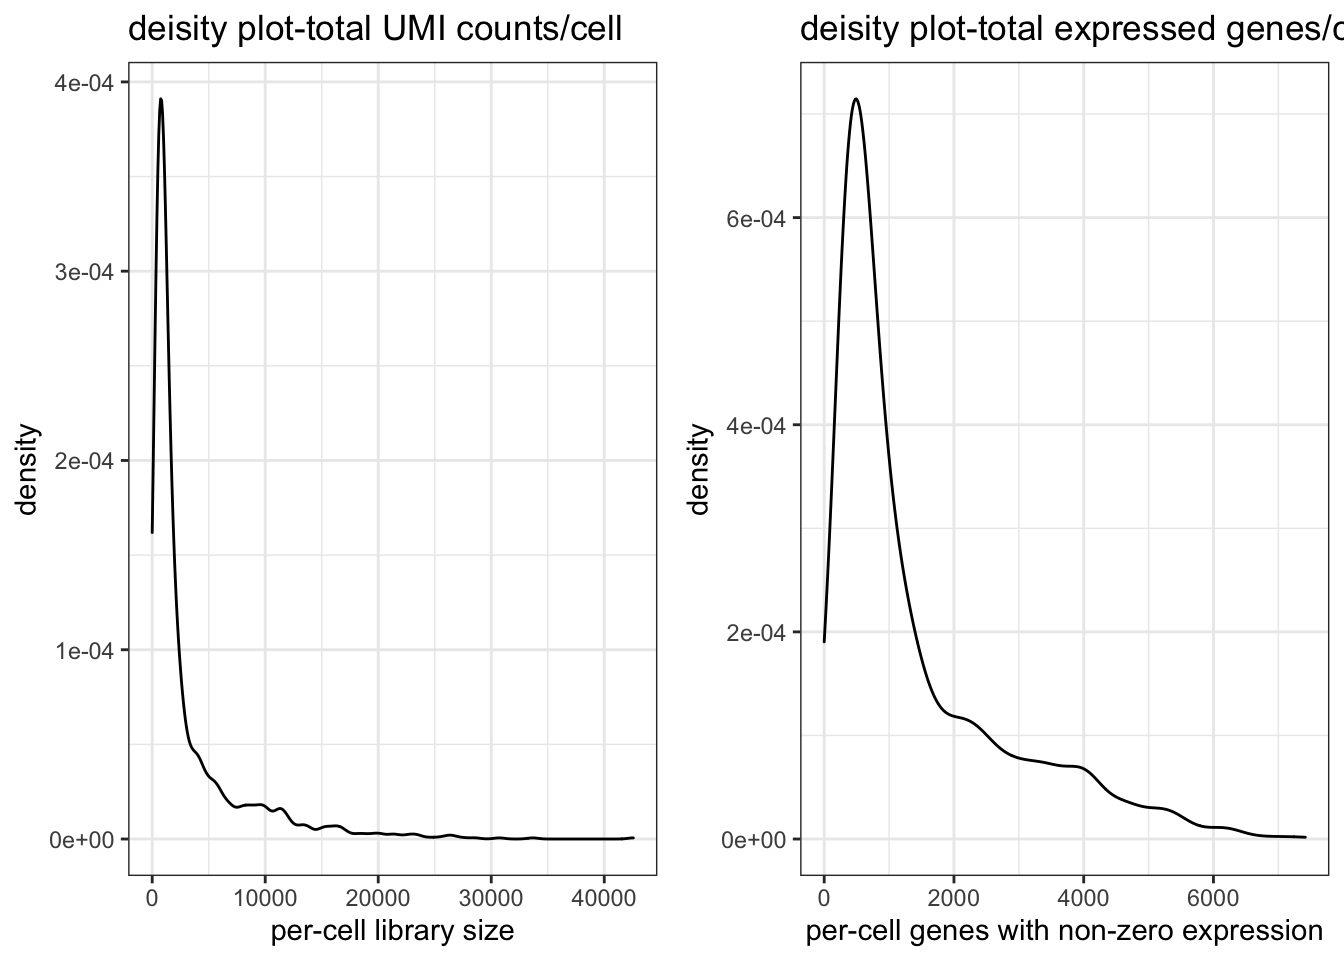
\includegraphics{HW10_JQI_files/figure-latex/unnamed-chunk-8-1.pdf}

\subsubsection{Describe in your own words what the two different
histograms show and what that means for the data at hand.
(2pts)}\label{describe-in-your-own-words-what-the-two-different-histograms-show-and-what-that-means-for-the-data-at-hand.-2pts}

SUM :: distribution of per-cell library size in the experiment\\
Detected :: distribution of per-cell genes with non-zero expression

\subsection{\texorpdfstring{For another extra-credit point, you could
generate the histogram for ``\% mitochondrial
reads''.}{For another extra-credit point, you could generate the histogram for \% mitochondrial reads.}}\label{for-another-extra-credit-point-you-could-generate-the-histogram-for-mitochondrial-reads.}

Note: You may find that the histograms are not as informative as you had
hoped. You may find the combination of violin plots (geom\_violin()) and
beeswarm plots (ggbeeswarm::geom\_quasirandom(alpha = 0.5)) more
helpful. More details on beeswarm plots can be found here.

\begin{Shaded}
\begin{Highlighting}[]
\KeywordTok{ggplot}\NormalTok{(per.cell}\OperatorTok\KeywordTok{data.frame}\NormalTok{())}\OperatorTok{+}
\StringTok{  }\KeywordTok{geom_density}\NormalTok{(}\KeywordTok{aes}\NormalTok{(subsets_Mito_percent))}\OperatorTok{+}
\StringTok{  }\KeywordTok{theme_bw}\NormalTok{()}\OperatorTok{+}
\StringTok{  }\KeywordTok{ggtitle}\NormalTok{(}\StringTok{"deisity plot-total Mito_percent counts/cell"}\NormalTok{)}\OperatorTok{+}
\StringTok{  }\KeywordTok{xlab}\NormalTok{(}\StringTok{"Mito_percent counts/cell"}\NormalTok{) ->}\StringTok{ }\NormalTok{p1}

\KeywordTok{ggplot}\NormalTok{(per.cell}\OperatorTok\KeywordTok{data.frame}\NormalTok{())}\OperatorTok{+}
\StringTok{  }\KeywordTok{geom_violin}\NormalTok{(}\KeywordTok{aes}\NormalTok{(}\DataTypeTok{y =}\NormalTok{ subsets_Mito_percent, }\DataTypeTok{x =} \DecValTok{1}\NormalTok{), }\DataTypeTok{trim =}\NormalTok{ F)}\OperatorTok{+}
\StringTok{  }\KeywordTok{theme_bw}\NormalTok{()}\OperatorTok{+}
\StringTok{  }\KeywordTok{ggtitle}\NormalTok{(}\StringTok{"violin plot-total Mito_percent counts/cell"}\NormalTok{)}\OperatorTok{+}
\StringTok{  }\KeywordTok{xlab}\NormalTok{(}\StringTok{"Mito_percent counts/cell"}\NormalTok{) ->}\StringTok{ }\NormalTok{p2}

\NormalTok{gridExtra}\OperatorTok{::}\KeywordTok{grid.arrange}\NormalTok{(p1, p2, }\DataTypeTok{ncol =} \DecValTok{2}\NormalTok{)}
\end{Highlighting}
\end{Shaded}

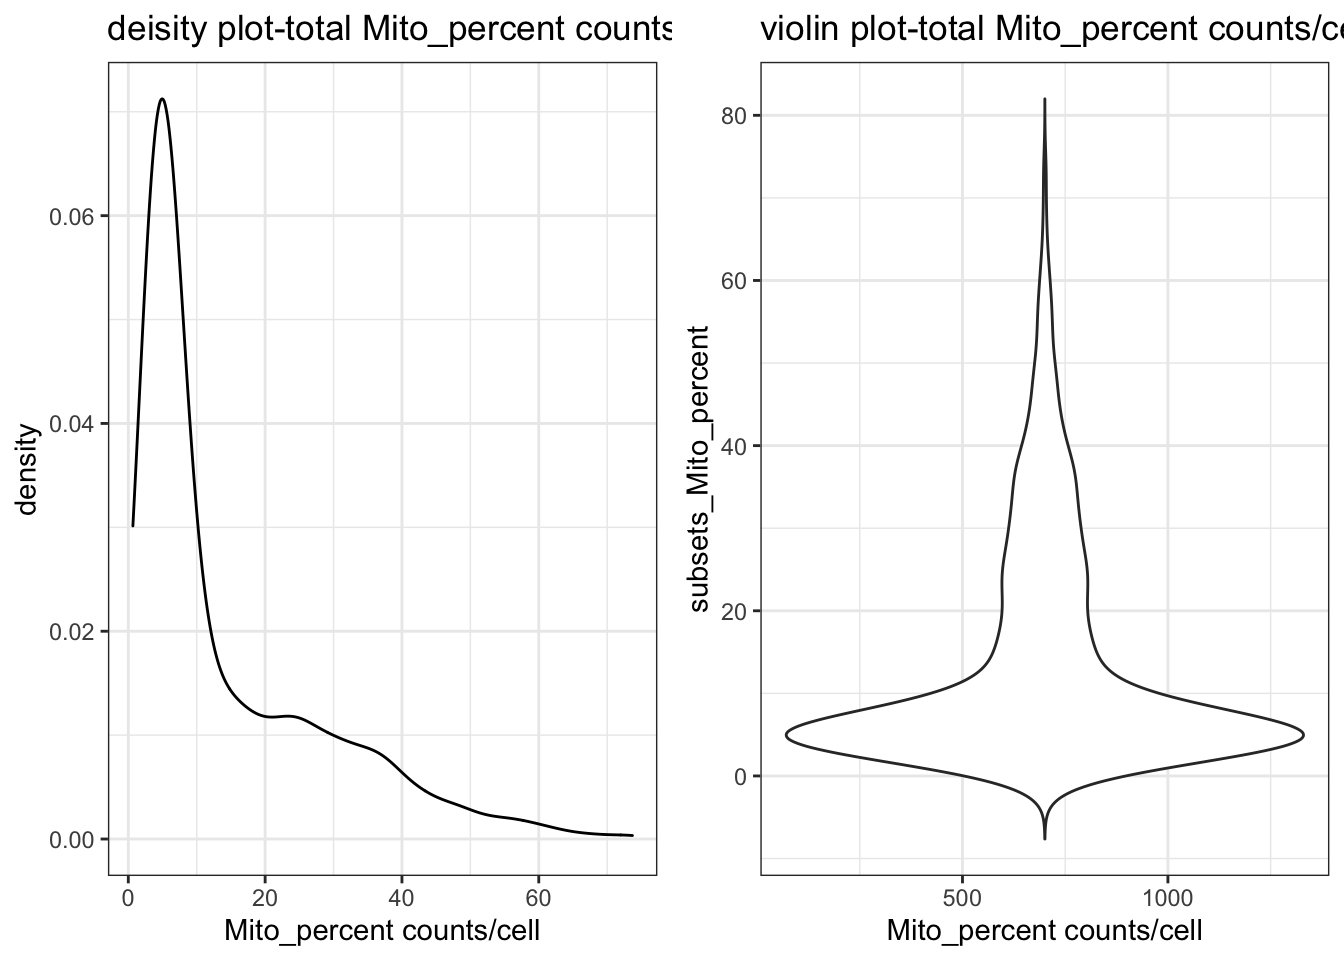
\includegraphics{HW10_JQI_files/figure-latex/unnamed-chunk-9-1.pdf}

\subsubsection{Decide on some threshold for either QC parameter and
remove the corresponding cells.
(1pt)}\label{decide-on-some-threshold-for-either-qc-parameter-and-remove-the-corresponding-cells.-1pt}

outlier threshod:\\
library size greater than 2times mads\\
non zero EG lower than 3 times mads\\
mito precentage greater than 3 times mads

\begin{Shaded}
\begin{Highlighting}[]
\KeywordTok{test_outlier}\NormalTok{(sce)}
\end{Highlighting}
\end{Shaded}

\includegraphics{HW10_JQI_files/figure-latex/unnamed-chunk-11-1.pdf}

\begin{Shaded}
\begin{Highlighting}[]
\NormalTok{### filtering low quality assay}
\CommentTok{#reasons <- quickPerCellQC(per.cell, percent_subsets=c("subsets_Mito_percent"))}
\CommentTok{#sce$discard <- reasons$discard}
\CommentTok{#colData(sce) <- cbind(colData(sce), per.cell)}
\CommentTok{#sum(reasons$discard)}
\CommentTok{#plot(per.cell$detected, per.cell$subsets_Mito_percent, col = ifelse(reasons$discard, "red", "black"),}
\CommentTok{#     main = "visualize outlier by quickPerCellQC()")}

\NormalTok{libsize.drop <-}\StringTok{ }\KeywordTok{isOutlier}\NormalTok{(per.cell}\OperatorTok{$}\NormalTok{sum, }\DataTypeTok{nmads=}\DecValTok{2}\NormalTok{, }\DataTypeTok{type=}\StringTok{"both"}\NormalTok{, }\DataTypeTok{log=}\NormalTok{T)}
\NormalTok{feature.drop <-}\StringTok{ }\KeywordTok{isOutlier}\NormalTok{(per.cell}\OperatorTok{$}\NormalTok{detected, }\DataTypeTok{nmads=}\DecValTok{3}\NormalTok{, }\DataTypeTok{type=}\StringTok{"both"}\NormalTok{, }\DataTypeTok{log=}\NormalTok{T)}
\NormalTok{mito.drop <-}\StringTok{ }\KeywordTok{isOutlier}\NormalTok{(per.cell}\OperatorTok{$}\NormalTok{subsets_Mito_percent, }\DataTypeTok{nmads=}\DecValTok{3}\NormalTok{, }\DataTypeTok{type=}\StringTok{"both"}\NormalTok{)}
\NormalTok{sce}\OperatorTok{$}\NormalTok{discard <-}\StringTok{ }\NormalTok{(libsize.drop }\OperatorTok{|}\StringTok{ }\NormalTok{feature.drop }\OperatorTok{|}\StringTok{ }\NormalTok{mito.drop )}
\KeywordTok{sum}\NormalTok{(sce}\OperatorTok{$}\NormalTok{discard) }\OperatorTok{/}\StringTok{ }\NormalTok{sce}\OperatorTok{@}\NormalTok{colData}\OperatorTok{@}\NormalTok{nrows}
\end{Highlighting}
\end{Shaded}

\begin{verbatim}
## [1] 0.2964286
\end{verbatim}

\begin{Shaded}
\begin{Highlighting}[]
\KeywordTok{plot}\NormalTok{(per.cell}\OperatorTok{$}\NormalTok{detected, per.cell}\OperatorTok{$}\NormalTok{subsets_Mito_percent, }\DataTypeTok{col =} \KeywordTok{ifelse}\NormalTok{(sce}\OperatorTok{$}\NormalTok{discard, }\StringTok{"red"}\NormalTok{, }\StringTok{"black"}\NormalTok{),}
     \DataTypeTok{main =} \StringTok{"visualize outlier by quickPerCellQC()"}\NormalTok{)}
\end{Highlighting}
\end{Shaded}

\includegraphics{HW10_JQI_files/figure-latex/unnamed-chunk-12-1.pdf}

\begin{Shaded}
\begin{Highlighting}[]
\KeywordTok{colData}\NormalTok{(sce) <-}\StringTok{ }\KeywordTok{cbind}\NormalTok{(}\KeywordTok{colData}\NormalTok{(sce), per.cell)}
\NormalTok{sce <-}\StringTok{ }\NormalTok{sce[,}\OperatorTok{!}\NormalTok{sce}\OperatorTok{$}\NormalTok{discard]}
\NormalTok{filtered <-}\StringTok{ }\KeywordTok{as.matrix}\NormalTok{(}\KeywordTok{assay}\NormalTok{(sce, }\StringTok{"counts"}\NormalTok{))}
\end{Highlighting}
\end{Shaded}

\subsubsection{Using the filtered data set, normalize the counts using
scran and scater and judge whether the size factors calculated by
computeSumFactors show the expected behavior as shown in Figure 6 of the
simpleSingleCell workflow.
(1pt)}\label{using-the-filtered-data-set-normalize-the-counts-using-scran-and-scater-and-judge-whether-the-size-factors-calculated-by-computesumfactors-show-the-expected-behavior-as-shown-in-figure-6-of-the-simplesinglecell-workflow.-1pt}

\begin{Shaded}
\begin{Highlighting}[]
\CommentTok{#sum(nexprs(filtered, byrow=TRUE) == 0 )}
\NormalTok{keep_feature <-}\StringTok{ }\KeywordTok{nexprs}\NormalTok{(filtered, }\DataTypeTok{byrow=}\OtherTok{TRUE}\NormalTok{) }\OperatorTok{>}\StringTok{ }\DecValTok{0}
\NormalTok{sce <-}\StringTok{ }\NormalTok{sce[keep_feature,]}
\CommentTok{#dim(example_sce)}
\NormalTok{sce <-}\StringTok{ }\KeywordTok{logNormCounts}\NormalTok{(sce, }\DataTypeTok{name =} \StringTok{"scater"}\NormalTok{)}


\NormalTok{clusters <-}\StringTok{ }\KeywordTok{quickCluster}\NormalTok{(sce)}
\CommentTok{#summary(sizeFactors(sce))}
\NormalTok{filtered_sf <-}\StringTok{ }\KeywordTok{computeSumFactors}\NormalTok{(}\KeywordTok{as.matrix}\NormalTok{(}\KeywordTok{assay}\NormalTok{(sce, }\StringTok{"counts"}\NormalTok{)), }\DataTypeTok{clusters=}\NormalTok{clusters, }\DataTypeTok{assay.type =} \StringTok{"SingleCellExperiment"}\NormalTok{)}
\NormalTok{sce <-}\StringTok{ }\KeywordTok{logNormCounts}\NormalTok{(sce, }\DataTypeTok{name =} \StringTok{"scran"}\NormalTok{, }\DataTypeTok{size_factors =}\NormalTok{ filtered_sf)}


\KeywordTok{plot}\NormalTok{(}\KeywordTok{colSums}\NormalTok{(}\DataTypeTok{x =} \KeywordTok{as.matrix}\NormalTok{(}\KeywordTok{assay}\NormalTok{(sce, }\StringTok{"counts"}\NormalTok{))),}\DataTypeTok{y=} \KeywordTok{sizeFactors}\NormalTok{(sce), }\DataTypeTok{log=}\StringTok{"xy"}\NormalTok{, }
     \DataTypeTok{xlab =} \StringTok{"log library size"}\NormalTok{)}
\end{Highlighting}
\end{Shaded}

\includegraphics{HW10_JQI_files/figure-latex/unnamed-chunk-13-1.pdf}

\begin{Shaded}
\begin{Highlighting}[]
\KeywordTok{assay}\NormalTok{(sce, }\StringTok{"scran"}\NormalTok{)}\OperatorTok
\StringTok{  }\KeywordTok{cbind.data.frame}\NormalTok{(}\DataTypeTok{RS =} \KeywordTok{rowSums}\NormalTok{(}\KeywordTok{assay}\NormalTok{(sce, }\StringTok{"scran"}\NormalTok{))) }\OperatorTok
\StringTok{  }\NormalTok{dplyr}\OperatorTok{::}\KeywordTok{arrange}\NormalTok{(}\KeywordTok{desc}\NormalTok{(RS))}\OperatorTok
\StringTok{  }\KeywordTok{head}\NormalTok{(}\DecValTok{3}\NormalTok{)}\OperatorTok
\StringTok{  }\KeywordTok{rbind.data.frame}\NormalTok{(}\DataTypeTok{Log_seq_depth =} \KeywordTok{assay}\NormalTok{(sce, }\StringTok{"scran"}\NormalTok{)}\OperatorTok\KeywordTok{colSums}\NormalTok{()}\OperatorTok\KeywordTok{log}\NormalTok{())}\OperatorTok
\StringTok{  }\NormalTok{data.table}\OperatorTok{::}\KeywordTok{transpose}\NormalTok{()}\OperatorTok
\StringTok{  }\NormalTok{tidyr}\OperatorTok{::}\KeywordTok{gather}\NormalTok{(}\OperatorTok{-}\NormalTok{V4, }\DataTypeTok{key =} \StringTok{"gene"}\NormalTok{, }\DataTypeTok{value =} \StringTok{"expression"}\NormalTok{)}\OperatorTok
\StringTok{  }\KeywordTok{ggplot}\NormalTok{(}\KeywordTok{aes}\NormalTok{(V4, }\KeywordTok{log}\NormalTok{(expression), }\DataTypeTok{color =}\NormalTok{ gene))}\OperatorTok{+}
\StringTok{  }\KeywordTok{geom_point}\NormalTok{()}\OperatorTok{+}
\StringTok{  }\KeywordTok{geom_smooth}\NormalTok{(}\DataTypeTok{method =} \StringTok{"lm"}\NormalTok{)}\OperatorTok{+}
\StringTok{  }\KeywordTok{ylim}\NormalTok{(}\KeywordTok{c}\NormalTok{(}\DecValTok{0}\NormalTok{,}\DecValTok{4}\NormalTok{))}\OperatorTok{+}
\StringTok{  }\KeywordTok{theme_bw}\NormalTok{()}\OperatorTok{+}
\StringTok{  }\KeywordTok{ggtitle}\NormalTok{(}\StringTok{"scran-adjustedSizeFactor"}\NormalTok{)->}\StringTok{ }\NormalTok{p1}
  

\KeywordTok{assay}\NormalTok{(sce, }\StringTok{"scater"}\NormalTok{)}\OperatorTok
\StringTok{  }\KeywordTok{cbind.data.frame}\NormalTok{(}\DataTypeTok{RS =} \KeywordTok{rowSums}\NormalTok{(}\KeywordTok{assay}\NormalTok{(sce, }\StringTok{"scater"}\NormalTok{))) }\OperatorTok
\StringTok{  }\NormalTok{dplyr}\OperatorTok{::}\KeywordTok{arrange}\NormalTok{(}\KeywordTok{desc}\NormalTok{(RS))}\OperatorTok
\StringTok{  }\KeywordTok{head}\NormalTok{(}\DecValTok{3}\NormalTok{)}\OperatorTok
\StringTok{  }\KeywordTok{rbind.data.frame}\NormalTok{(}\DataTypeTok{Log_seq_depth =} \KeywordTok{assay}\NormalTok{(sce, }\StringTok{"scater"}\NormalTok{)}\OperatorTok\KeywordTok{colSums}\NormalTok{()}\OperatorTok\KeywordTok{log}\NormalTok{())}\OperatorTok
\StringTok{  }\NormalTok{data.table}\OperatorTok{::}\KeywordTok{transpose}\NormalTok{()}\OperatorTok
\StringTok{  }\NormalTok{tidyr}\OperatorTok{::}\KeywordTok{gather}\NormalTok{(}\OperatorTok{-}\NormalTok{V4, }\DataTypeTok{key =} \StringTok{"gene"}\NormalTok{, }\DataTypeTok{value =} \StringTok{"expression"}\NormalTok{)}\OperatorTok
\StringTok{  }\KeywordTok{ggplot}\NormalTok{(}\KeywordTok{aes}\NormalTok{(V4, }\KeywordTok{log}\NormalTok{(expression), }\DataTypeTok{color =}\NormalTok{ gene))}\OperatorTok{+}
\StringTok{  }\KeywordTok{geom_point}\NormalTok{()}\OperatorTok{+}
\StringTok{  }\KeywordTok{geom_smooth}\NormalTok{(}\DataTypeTok{method =} \StringTok{"lm"}\NormalTok{)}\OperatorTok{+}
\StringTok{  }\KeywordTok{ylim}\NormalTok{(}\KeywordTok{c}\NormalTok{(}\DecValTok{0}\NormalTok{,}\DecValTok{4}\NormalTok{))}\OperatorTok{+}
\StringTok{  }\KeywordTok{theme_bw}\NormalTok{()}\OperatorTok{+}
\StringTok{  }\KeywordTok{ggtitle}\NormalTok{(}\StringTok{"scater-globalSizeFactor"}\NormalTok{) ->}\StringTok{ }\NormalTok{p2}

\NormalTok{gridExtra}\OperatorTok{::}\KeywordTok{grid.arrange}\NormalTok{(p1, p2, }\DataTypeTok{ncol =} \DecValTok{2}\NormalTok{)}
\end{Highlighting}
\end{Shaded}

\includegraphics{HW10_JQI_files/figure-latex/unnamed-chunk-13-2.pdf}
instead of using 1 global size factor, scran calculated size factor in
adjust to library size of each cell. however as inspected, nither scran
or scater normalize count in adjust to expression level of each genes.
will compare with Seurat below.

\subsubsection{How can you access the normalized data matrix?
(0.5pt)}\label{how-can-you-access-the-normalized-data-matrix-0.5pt}

\begin{Shaded}
\begin{Highlighting}[]
\KeywordTok{assayNames}\NormalTok{(sce)}
\end{Highlighting}
\end{Shaded}

\begin{verbatim}
## [1] "counts" "scater" "scran"
\end{verbatim}

\subsubsection{2. scRNA-seq data wrangling in R using Seurat.
(8.5pts)}\label{scrna-seq-data-wrangling-in-r-using-seurat.-8.5pts}

\subsubsection{Seurat can be installed via the usual install.packages
routine.}\label{seurat-can-be-installed-via-the-usual-install.packages-routine.}

\subsubsection{Create a Seurat object.
(1pt)}\label{create-a-seurat-object.-1pt}

\begin{Shaded}
\begin{Highlighting}[]
\NormalTok{Sobj <-}\StringTok{ }\KeywordTok{CreateSeuratObject}\NormalTok{(}\DataTypeTok{counts =}\NormalTok{ Count_Matrix)}
\end{Highlighting}
\end{Shaded}

\begin{verbatim}
## Warning: Feature names cannot have underscores ('_'), replacing with dashes
## ('-')
\end{verbatim}

\subsubsection{Perform the same filtering that you chose to do on the
SCE object.
(1pt)}\label{perform-the-same-filtering-that-you-chose-to-do-on-the-sce-object.-1pt}

\begin{Shaded}
\begin{Highlighting}[]
\NormalTok{Sobj[[}\StringTok{"percent.mt"}\NormalTok{]] <-}\StringTok{ }\KeywordTok{PercentageFeatureSet}\NormalTok{(Sobj, }\DataTypeTok{pattern =} \StringTok{"^MT"}\NormalTok{)}
\CommentTok{#VlnPlot(Sobj, features = c("nFeature_RNA", "nCount_RNA", "percent.mt"), ncol = 3)}
\NormalTok{plot1 <-}\StringTok{ }\KeywordTok{FeatureScatter}\NormalTok{(Sobj, }\DataTypeTok{feature1 =} \StringTok{"nCount_RNA"}\NormalTok{, }\DataTypeTok{feature2 =} \StringTok{"percent.mt"}\NormalTok{)}
\NormalTok{plot2 <-}\StringTok{ }\KeywordTok{FeatureScatter}\NormalTok{(Sobj, }\DataTypeTok{feature1 =} \StringTok{"nCount_RNA"}\NormalTok{, }\DataTypeTok{feature2 =} \StringTok{"nFeature_RNA"}\NormalTok{)}
\NormalTok{gridExtra}\OperatorTok{::}\KeywordTok{grid.arrange}\NormalTok{(plot1, plot2, }\DataTypeTok{ncol =} \DecValTok{2}\NormalTok{)}
\end{Highlighting}
\end{Shaded}

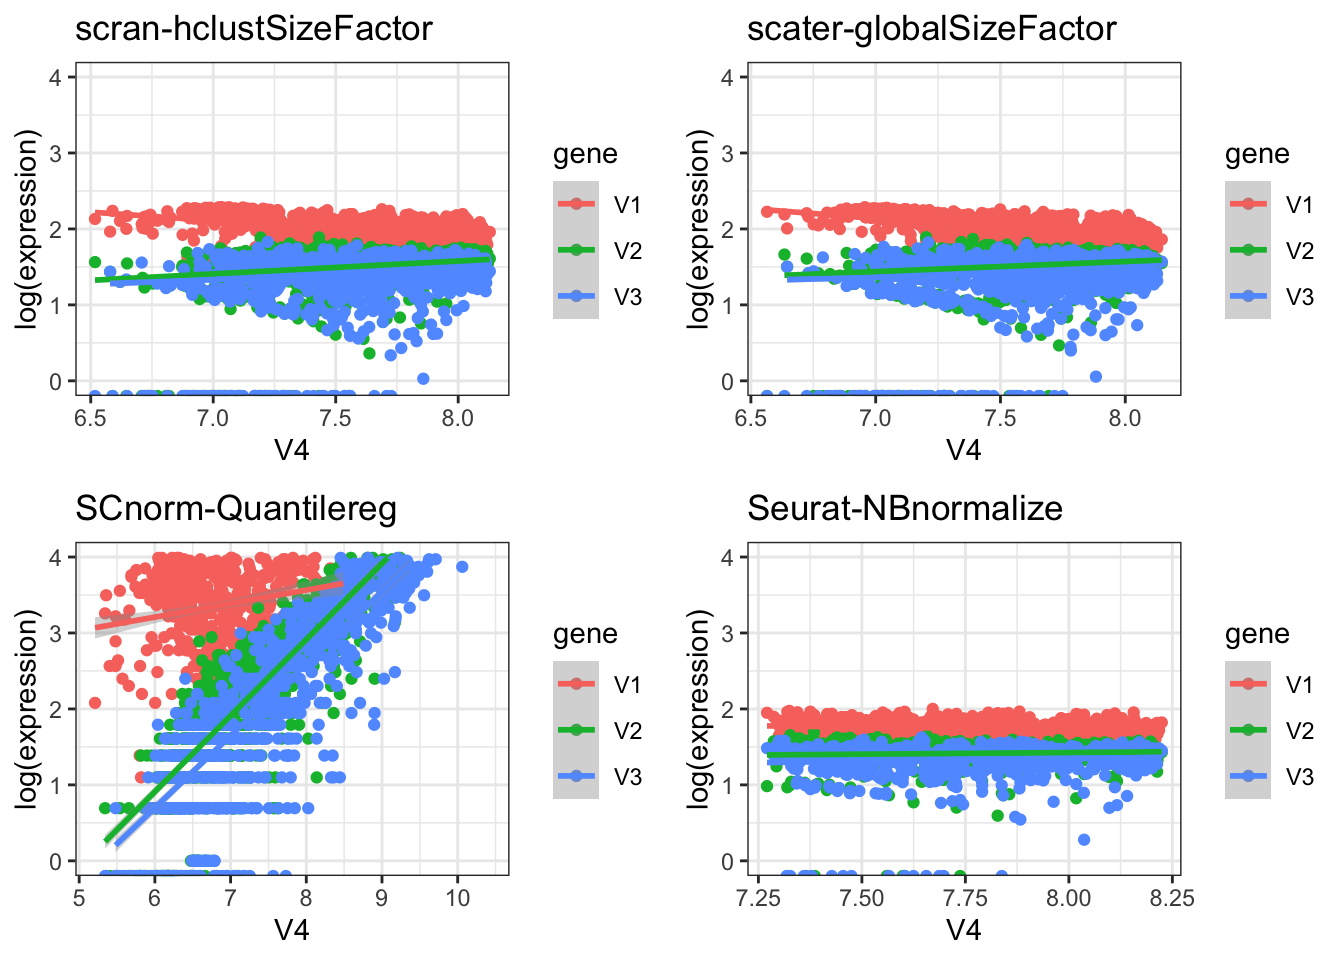
\includegraphics{HW10_JQI_files/figure-latex/unnamed-chunk-16-1.pdf}

\begin{Shaded}
\begin{Highlighting}[]
\NormalTok{Sobj <-}\StringTok{ }\KeywordTok{subset}\NormalTok{(Sobj, }\DataTypeTok{subset =}\NormalTok{ nFeature_RNA }\OperatorTok{>}\StringTok{ }\DecValTok{500} \OperatorTok{&}\StringTok{ }\NormalTok{nFeature_RNA }\OperatorTok{<}\StringTok{ }\DecValTok{3000} \OperatorTok{&}\StringTok{ }\NormalTok{percent.mt }\OperatorTok{<}\StringTok{ }\DecValTok{20}\NormalTok{)}
\CommentTok{#VlnPlot(Sobj, features = c("nFeature_RNA", "nCount_RNA", "percent.mt"), ncol = 3)}
\end{Highlighting}
\end{Shaded}

\subsubsection{Normalize the data using scTransform
(1pt)}\label{normalize-the-data-using-sctransform-1pt}

\begin{Shaded}
\begin{Highlighting}[]
\NormalTok{Sobj <-}\StringTok{ }\KeywordTok{NormalizeData}\NormalTok{(Sobj)}
\end{Highlighting}
\end{Shaded}

\subsubsection{How can you access the normalized data matrix, i.e.~the
matrix of Pearson residuals?
(0.5pts)}\label{how-can-you-access-the-normalized-data-matrix-i.e.the-matrix-of-pearson-residuals-0.5pts}

\begin{Shaded}
\begin{Highlighting}[]
\NormalTok{Sobj}\OperatorTok{@}\NormalTok{assays}\OperatorTok{$}\NormalTok{RNA}\OperatorTok{@}\NormalTok{data}
\end{Highlighting}
\end{Shaded}

\begin{Shaded}
\begin{Highlighting}[]
\NormalTok{Sobj}\OperatorTok{@}\NormalTok{assays}\OperatorTok{$}\NormalTok{RNA}\OperatorTok{@}\NormalTok{data}\OperatorTok
\StringTok{  }\KeywordTok{cbind.data.frame}\NormalTok{(}\DataTypeTok{RS =} \KeywordTok{rowSums}\NormalTok{(Sobj}\OperatorTok{@}\NormalTok{assays}\OperatorTok{$}\NormalTok{RNA}\OperatorTok{@}\NormalTok{data)) }\OperatorTok
\StringTok{  }\NormalTok{dplyr}\OperatorTok{::}\KeywordTok{arrange}\NormalTok{(}\KeywordTok{desc}\NormalTok{(RS))}\OperatorTok
\StringTok{  }\KeywordTok{head}\NormalTok{(}\DecValTok{3}\NormalTok{)}\OperatorTok
\StringTok{  }\KeywordTok{rbind.data.frame}\NormalTok{(}\DataTypeTok{Log_seq_depth =}\NormalTok{ Sobj}\OperatorTok{@}\NormalTok{assays}\OperatorTok{$}\NormalTok{RNA}\OperatorTok{@}\NormalTok{data }\OperatorTok\KeywordTok{colSums}\NormalTok{()}\OperatorTok\KeywordTok{log}\NormalTok{())}\OperatorTok
\StringTok{  }\NormalTok{data.table}\OperatorTok{::}\KeywordTok{transpose}\NormalTok{()}\OperatorTok
\StringTok{  }\NormalTok{tidyr}\OperatorTok{::}\KeywordTok{gather}\NormalTok{(}\OperatorTok{-}\NormalTok{V4, }\DataTypeTok{key =} \StringTok{"gene"}\NormalTok{, }\DataTypeTok{value =} \StringTok{"expression"}\NormalTok{)}\OperatorTok
\StringTok{  }\KeywordTok{ggplot}\NormalTok{(}\KeywordTok{aes}\NormalTok{(V4, }\KeywordTok{log}\NormalTok{(expression), }\DataTypeTok{color =}\NormalTok{ gene))}\OperatorTok{+}
\StringTok{  }\KeywordTok{geom_point}\NormalTok{()}\OperatorTok{+}
\StringTok{  }\KeywordTok{geom_smooth}\NormalTok{(}\DataTypeTok{method =} \StringTok{"lm"}\NormalTok{)}\OperatorTok{+}
\StringTok{  }\KeywordTok{ylim}\NormalTok{(}\KeywordTok{c}\NormalTok{(}\DecValTok{0}\NormalTok{,}\DecValTok{4}\NormalTok{))}\OperatorTok{+}
\StringTok{  }\KeywordTok{theme_bw}\NormalTok{()}\OperatorTok{+}
\StringTok{  }\KeywordTok{ggtitle}\NormalTok{(}\StringTok{"Seurat-NBnormalize"}\NormalTok{)->p3}


\NormalTok{gridExtra}\OperatorTok{::}\KeywordTok{grid.arrange}\NormalTok{(p1, p2, p3, }\DataTypeTok{ncol =} \DecValTok{2}\NormalTok{, }\DataTypeTok{nrow =} \DecValTok{2}\NormalTok{)}
\end{Highlighting}
\end{Shaded}

\includegraphics{HW10_JQI_files/figure-latex/unnamed-chunk-19-1.pdf}
\#\#\#For the first 10 cells, do pairwise comparisons for each cell of
the normalized values from the Seurat object and the SCE object (scatter
plots are fine; you may want to check out the GGally package,
specifically the ggpairs function. We also recommend to remove genes
that have zero counts in all the samples). Explain what you see. (2pts)

\begin{Shaded}
\begin{Highlighting}[]
\CommentTok{#common cell idx}
\CommentTok{#Sobj@assays$RNA@data@Dimnames[[2]][cidx]}
\NormalTok{cidx <-}\StringTok{ }\KeywordTok{colnames}\NormalTok{(}\KeywordTok{assay}\NormalTok{(sce, }\StringTok{"scater"}\NormalTok{)) }\OperatorTok\StringTok{ }\NormalTok{Sobj}\OperatorTok{@}\NormalTok{assays}\OperatorTok{$}\NormalTok{RNA}\OperatorTok{@}\NormalTok{data}\OperatorTok{@}\NormalTok{Dimnames[[}\DecValTok{2}\NormalTok{]][}\DecValTok{2}\OperatorTok{:}\DecValTok{11}\NormalTok{]}
\NormalTok{cidx <-}\StringTok{ }\KeywordTok{sort}\NormalTok{(Sobj}\OperatorTok{@}\NormalTok{assays}\OperatorTok{$}\NormalTok{RNA}\OperatorTok{@}\NormalTok{data}\OperatorTok{@}\NormalTok{Dimnames[[}\DecValTok{2}\NormalTok{]][cidx])}
\KeywordTok{length}\NormalTok{(cidx)}
\end{Highlighting}
\end{Shaded}

\begin{verbatim}
## [1] 10
\end{verbatim}

\begin{Shaded}
\begin{Highlighting}[]
\CommentTok{#common feature idx}
\NormalTok{commS_nonZero <-}\StringTok{ }\NormalTok{Sobj}\OperatorTok{@}\NormalTok{assays}\OperatorTok{$}\NormalTok{RNA}\OperatorTok{@}\NormalTok{data}\OperatorTok{@}\NormalTok{Dimnames[[}\DecValTok{1}\NormalTok{]][}\KeywordTok{which}\NormalTok{(}\KeywordTok{rowSums}\NormalTok{(Sobj}\OperatorTok{@}\NormalTok{assays}\OperatorTok{$}\NormalTok{RNA}\OperatorTok{@}\NormalTok{data[, cidx]) }\OperatorTok{!=}\StringTok{ }\DecValTok{0}\NormalTok{)]}
\KeywordTok{length}\NormalTok{(commS_nonZero)}
\end{Highlighting}
\end{Shaded}

\begin{verbatim}
## [1] 8154
\end{verbatim}

\begin{Shaded}
\begin{Highlighting}[]
\NormalTok{commRc <-}\StringTok{ }\KeywordTok{rownames}\NormalTok{(}\KeywordTok{assay}\NormalTok{(sce, }\StringTok{"scater"}\NormalTok{))[}\KeywordTok{which}\NormalTok{(}\KeywordTok{rownames}\NormalTok{(}\KeywordTok{assay}\NormalTok{(sce, }\StringTok{"scater"}\NormalTok{)) }\OperatorTok\StringTok{ }\NormalTok{commS_nonZero)]}
\NormalTok{commS_nonZero <-}\StringTok{ }\NormalTok{Sobj}\OperatorTok{@}\NormalTok{assays}\OperatorTok{$}\NormalTok{RNA}\OperatorTok{@}\NormalTok{data}\OperatorTok{@}\NormalTok{Dimnames[[}\DecValTok{1}\NormalTok{]][}\KeywordTok{which}\NormalTok{(Sobj}\OperatorTok{@}\NormalTok{assays}\OperatorTok{$}\NormalTok{RNA}\OperatorTok{@}\NormalTok{data}\OperatorTok{@}\NormalTok{Dimnames[[}\DecValTok{1}\NormalTok{]] }\OperatorTok\StringTok{ }\NormalTok{commRc)]}


\NormalTok{st <-}\StringTok{ }\KeywordTok{data.frame}\NormalTok{(}\DataTypeTok{geneid =}\NormalTok{ commS_nonZero,}
\NormalTok{           Sobj}\OperatorTok{@}\NormalTok{assays}\OperatorTok{$}\NormalTok{RNA}\OperatorTok{@}\NormalTok{data[commS_nonZero, cidx]) }
\CommentTok{#st$method = rep("seurat", nrow(st))}

\NormalTok{sc <-}\StringTok{ }\KeywordTok{data.frame}\NormalTok{(}\DataTypeTok{geneid =}\NormalTok{ commS_nonZero,}
                 \KeywordTok{assay}\NormalTok{(sce, }\StringTok{"scater"}\NormalTok{)[commS_nonZero , cidx])}
\NormalTok{sd <-}\StringTok{ }\KeywordTok{data.frame}\NormalTok{(}\DataTypeTok{geneid =}\NormalTok{ commS_nonZero,}
                 \KeywordTok{assay}\NormalTok{(sce, }\StringTok{"scran"}\NormalTok{)[commS_nonZero , cidx])}

\CommentTok{#sc$method = rep("scater", nrow(sc))}

\NormalTok{df1 <-}\StringTok{ }\KeywordTok{cbind.data.frame}\NormalTok{(}\DataTypeTok{seurat =} \KeywordTok{unlist}\NormalTok{(st[}\DecValTok{2}\OperatorTok{:}\DecValTok{11}\NormalTok{]),}
                        \DataTypeTok{scater =} \KeywordTok{unlist}\NormalTok{(sc[}\DecValTok{2}\OperatorTok{:}\DecValTok{11}\NormalTok{]),}
                        \DataTypeTok{scran =} \KeywordTok{unlist}\NormalTok{(sd[}\DecValTok{2}\OperatorTok{:}\DecValTok{11}\NormalTok{]),}
                        \DataTypeTok{sample =} \KeywordTok{rep}\NormalTok{(}\KeywordTok{colnames}\NormalTok{(st)[}\DecValTok{2}\OperatorTok{:}\DecValTok{11}\NormalTok{], }\DataTypeTok{each =} \KeywordTok{nrow}\NormalTok{(st))) }


\NormalTok{GGally}\OperatorTok{::}\KeywordTok{ggpairs}\NormalTok{(df1, }\DecValTok{1}\OperatorTok{:}\DecValTok{3}\NormalTok{, }\DataTypeTok{mapping =}\NormalTok{ ggplot2}\OperatorTok{::}\KeywordTok{aes}\NormalTok{(}\DataTypeTok{color =}\NormalTok{ sample))}
\end{Highlighting}
\end{Shaded}

\includegraphics{HW10_JQI_files/figure-latex/unnamed-chunk-20-1.pdf}

\emph{two packages workflow filtered dataset differently. scaret outlier
is set by standard dev from the mean; threshod in Seurat is more like
setting by eye-balling, though it appears to correct the bias caused by
depth difference}

\subsubsection{What is the difference between the function implemented
in scTransform and the integration routine that is described here and by
Stuart et al.?
(1pt}\label{what-is-the-difference-between-the-function-implemented-in-sctransform-and-the-integration-routine-that-is-described-here-and-by-stuart-et-al.-1pt}

scTransform model the expression of each gene as a negative binomial
random variable with a mean that depends on other variables. observed
UMI is transferd as of dispersion. it generated new assay slot with data
that with variance stabalization.

\subsubsection{3. Final question: what types of cells do you think
you're looking at? (1pt + 1 extra-credit
point)}\label{final-question-what-types-of-cells-do-you-think-youre-looking-at-1pt-1-extra-credit-point}

Hint: It is a fairly homogeneous population, i.e.~all cells would
probably be called the same cell name where cell name would be something
like ``skin cell''. Explain your reasoning!\\
The point is for your reasoning, there will be an extra-credit point if
you identify the cell type correctly.

\begin{Shaded}
\begin{Highlighting}[]
\NormalTok{gemean <-}\StringTok{ }\NormalTok{Sobj}\OperatorTok{@}\NormalTok{assays}\OperatorTok{$}\NormalTok{RNA}\OperatorTok{@}\NormalTok{data }\OperatorTok
\StringTok{  }\KeywordTok{rowSums}\NormalTok{() }\OperatorTok
\StringTok{  }\KeywordTok{sort}\NormalTok{(}\DataTypeTok{decreasing =}\NormalTok{ T) }

\NormalTok{top10 <-}\StringTok{ }\KeywordTok{head}\NormalTok{(gemean, }\DataTypeTok{n =} \DecValTok{10}\NormalTok{)}
\NormalTok{tail10 <-}\StringTok{ }\KeywordTok{tail}\NormalTok{(gemean, }\DataTypeTok{n =} \DecValTok{10}\NormalTok{)}

\KeywordTok{data.frame}\NormalTok{(}\DataTypeTok{geneid =} \KeywordTok{c}\NormalTok{(}\KeywordTok{names}\NormalTok{(top10), }\KeywordTok{names}\NormalTok{(tail10)),}
                  \DataTypeTok{meanGE =} \KeywordTok{c}\NormalTok{(top10, tail10))}\OperatorTok
\StringTok{  }\KeywordTok{mutate}\NormalTok{(}\DataTypeTok{geneid =} \KeywordTok{fct_reorder}\NormalTok{(geneid, meanGE)) ->df2}


\KeywordTok{ggplot}\NormalTok{(df2)}\OperatorTok{+}
\StringTok{  }\KeywordTok{geom_bar}\NormalTok{(}\KeywordTok{aes}\NormalTok{(}\DataTypeTok{y =}\NormalTok{ meanGE, }\DataTypeTok{x =}\NormalTok{ geneid), }\DataTypeTok{stat =} \StringTok{"identity"}\NormalTok{)}\OperatorTok{+}\StringTok{ }
\StringTok{  }\KeywordTok{theme}\NormalTok{(}\DataTypeTok{axis.text.x =} \KeywordTok{element_text}\NormalTok{(}\DataTypeTok{angle =} \DecValTok{90}\NormalTok{, }\DataTypeTok{hjust =} \DecValTok{1}\NormalTok{))}
\end{Highlighting}
\end{Shaded}

\includegraphics{HW10_JQI_files/figure-latex/unnamed-chunk-21-1.pdf}

\begin{Shaded}
\begin{Highlighting}[]
\KeywordTok{data}\NormalTok{(hpaNormalTissue)}
\NormalTok{gf <-}\StringTok{ }\KeywordTok{data.frame}\NormalTok{(}\DataTypeTok{Gene.name =}\NormalTok{ hpaNormalTissue}\OperatorTok{$}\NormalTok{Gene.name[}\KeywordTok{which}\NormalTok{(hpaNormalTissue}\OperatorTok{$}\NormalTok{Gene.name }\OperatorTok\StringTok{ }\KeywordTok{names}\NormalTok{(top10))])}

\NormalTok{queryreslt <-}\StringTok{ }
\StringTok{  }\NormalTok{gf }\OperatorTok
\StringTok{  }\KeywordTok{left_join}\NormalTok{(hpaNormalTissue, }\DataTypeTok{by =} \StringTok{"Gene.name"}\NormalTok{)}

\KeywordTok{table}\NormalTok{(queryreslt}\OperatorTok{$}\NormalTok{Cell.type)}\OperatorTok
\StringTok{  }\KeywordTok{data.frame}\NormalTok{()}\OperatorTok
\StringTok{  }\KeywordTok{arrange}\NormalTok{(}\KeywordTok{desc}\NormalTok{(Freq))}\OperatorTok
\StringTok{  }\KeywordTok{head}\NormalTok{(}\DecValTok{10}\NormalTok{)}
\end{Highlighting}
\end{Shaded}

\begin{verbatim}
##                           Var1 Freq
## 1              glandular cells 7765
## 2    squamous epithelial cells 1980
## 3                  fibroblasts 1188
## 4                  glial cells 1188
## 5               neuronal cells 1188
## 6                   adipocytes 1029
## 7  cells in endometrial stroma  792
## 8            endothelial cells  792
## 9        germinal center cells  792
## 10                    myocytes  792
\end{verbatim}

based on summarization of mean gene expression of the normalized data.
the genes are sorted by decreasing order of mean expression. the gene id
is queried from Human Protein Atlas R package. Cell type is matched with
the top 500 most expressed genes. contengency table is generated by
possible matatching cell types Grandular cells got the most hits.


\end{document}
